\let\negmedspace\undefined
\let\negthickspace\undefined
\documentclass[journal]{IEEEtran}
\usepackage[a5paper, margin=10mm, onecolumn]{geometry}
%\usepackage{lmodern} % Ensure lmodern is loaded for pdflatex
% \usepackage{tfrupee} % Include tfrupee package

\setlength{\headheight}{1cm} % Set the height of the header box
\setlength{\headsep}{0mm}     % Set the distance between the header box and the top of the text

\usepackage{gvv-book}
\usepackage{gvv}
\usepackage{cite}
\usepackage{amsmath,amssymb,amsfonts,amsthm}
\usepackage{algorithm}
\usepackage{algorithmic}
\usepackage{graphicx}
\usepackage{textcomp}
\usepackage{xcolor}
\usepackage{txfonts}
\usepackage{listings}
\usepackage{enumitem}
\usepackage{mathtools}
\usepackage{gensymb}
\usepackage{comment}
\usepackage[breaklinks=true]{hyperref}
\usepackage{tkz-euclide} 
\usepackage{listings}
% \usepackage{gvv}                                        
\def\inputGnumericTable{}                                 
\usepackage[latin1]{inputenc}                                
\usepackage{color}                                            
\usepackage{array}                                            
\usepackage{longtable}                
\usepackage{calc}                                             
\usepackage{multirow}                                         
\usepackage{hhline}                                           
\usepackage{ifthen}                                           
\usepackage{lscape}
% \usepackage{algpseudocode}
\begin{document}

\bibliographystyle{IEEEtran}
\vspace{3cm}

\title{Activity 1} 
\author{S A Aravind Eswar and Eshan Sharma}
{\let\newpage\relax\maketitle}

\section{Aim}
\begin{enumerate}
    \item At least 6 Lissajous figures should be plotted on the oscilloscope and justify the pattern you see on CRO with theory.
    \item How do you capture one-time event on CRO -  show with an example
\end{enumerate}

\section{Apparatus Required}
\begin{enumerate}
    \item Oscilloscope (Digital with two channels)
    \item Function Generator (with two channels)
    \item Two probes
    \item Two connection wires
\end{enumerate}

\section{Theory}
\subsection{Lissajous figuers}

Lissajous cures are defined as a parametric curve given by,
\begin{align}
    x = A\sin(at+\delta),\,y = B\sin(bt)
\end{align}

which describe the superposition of two perpendicular oscillations in x and y directions of different angular frequency.

We can use an oscilloscope to project a Lissajous curve. We can send signal 1 to the top-bottom plates of the oscilloscope and signal 2 to the left-right plates. This achieves the given parametric equation.

% \subsection{Capturing a moment}

% We can use a Digital 

\section{Procedure}
\subsection{Lissajous figures}
\begin{enumerate}
    \item Take a Function generator and an oscilloscope with 2 channels.
    \item Connect channel 1 of function generator with channel 1 of the oscilloscope and channel 2 of function generator to channel 2 of oscilloscope.
    \item Set channel 1 and channel 2 of the function generator to desired functions
    \item Change the display mode of the oscilloscope to x-y mode
    \item Observe the shapes produced by the oscilloscope
\end{enumerate}

\subsection{Capturing an event}
\begin{enumerate}
    \item Use the function generator to trigger a pulse signal on manual trigger
    \item Set the trigger level in the CRO to an appropriate level (0.1V)
    \item Set the Run control to single
    \item Observe that it says \texttt{WAIT} on the top left of the CRO
    \item Trigger the signal from the function generator
    \item Observe the CRO output
\end{enumerate}

\section{Observarion}
\subsection{Lissajous curves}
\begin{enumerate}
    %1
    \item \begin{align*}
        x = 5\sin\brak{\frac{2\pi}{3}t},\,y = 5\sin\brak{\frac{2\pi}{3}t}
    \end{align*}
    \begin{figure}[h]
        \centering
        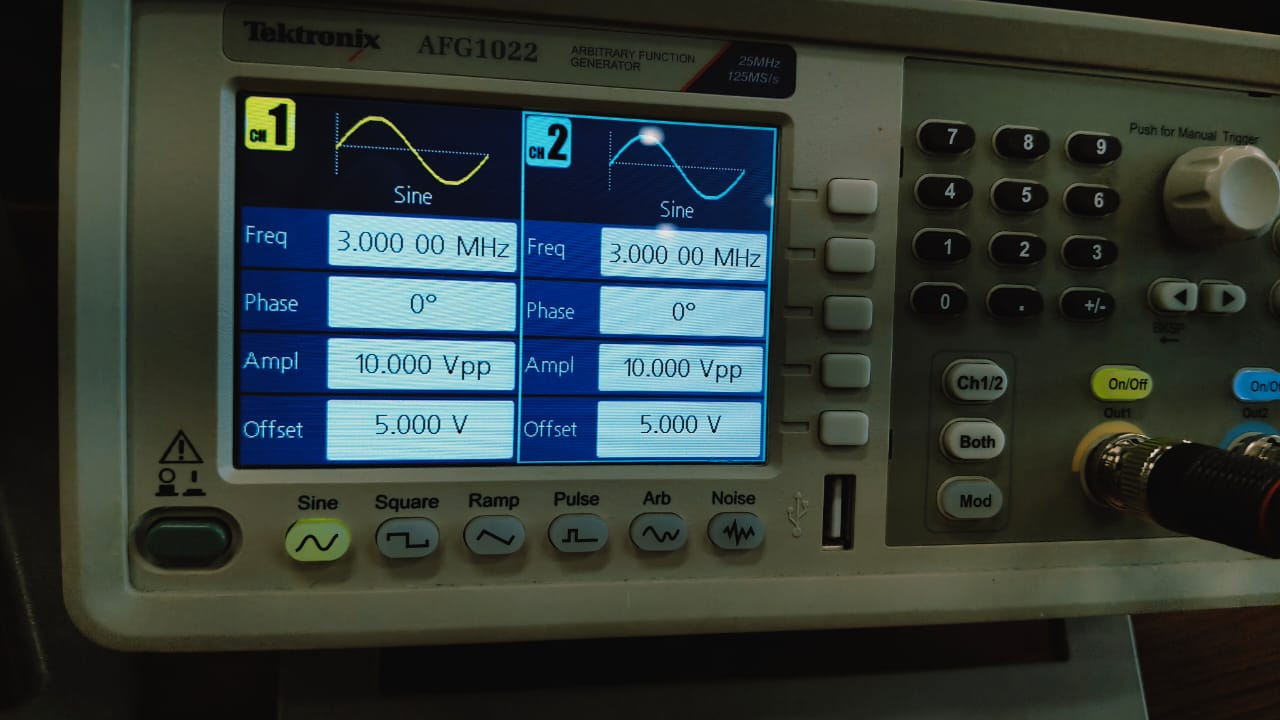
\includegraphics[width=0.7\columnwidth]{pics/WhatsApp Image 2025-01-15 at 23.32.36.jpeg}
        \caption{Input from function generator}
    \end{figure}
    \begin{figure}[h]
        \centering
        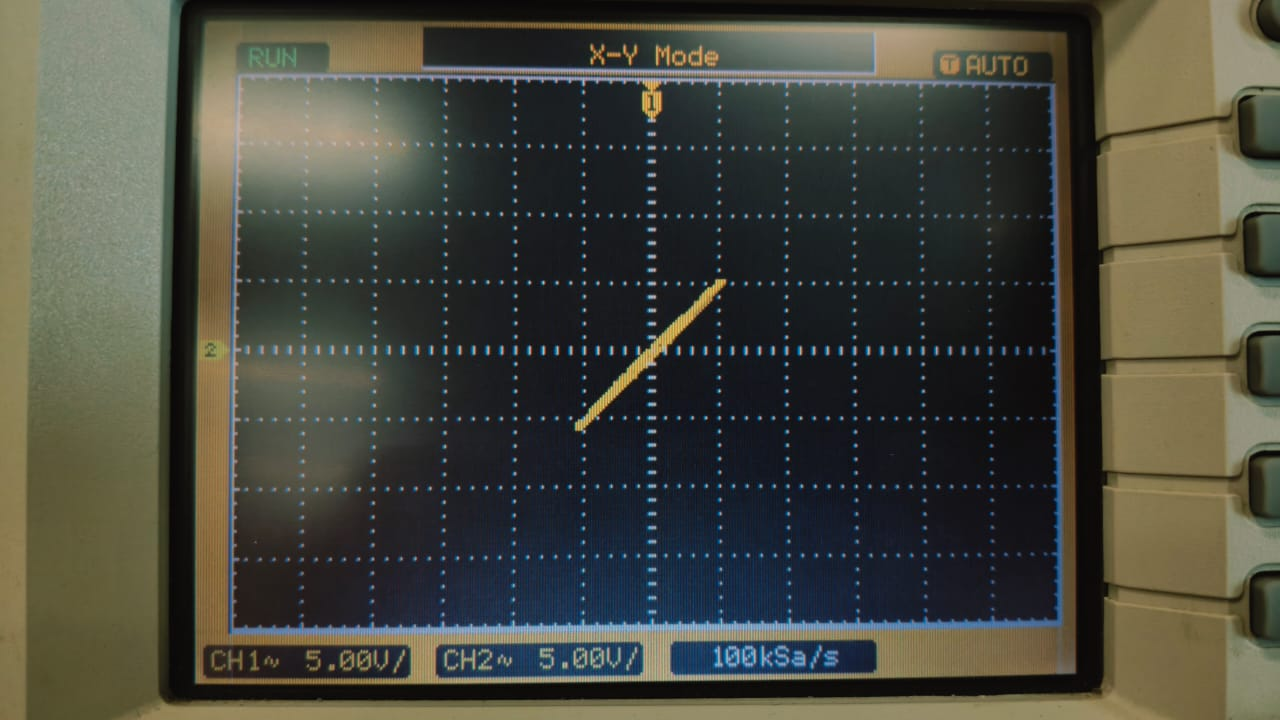
\includegraphics[width=0.7\columnwidth]{pics/WhatsApp Image 2025-01-15 at 23.32.36(1).jpeg}
        \caption{Output on CRO}
    \end{figure}
    \begin{figure}[H]
        \centering
        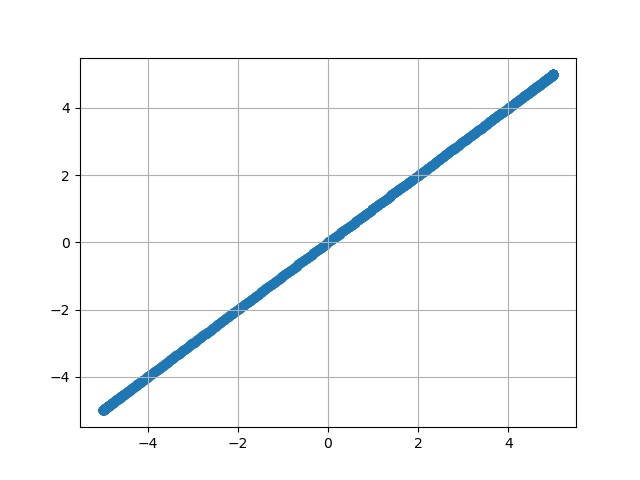
\includegraphics[width=0.7\columnwidth]{figs/fig1.png}
        \caption{Theoretical PLot}
    \end{figure}
    %2
    \item \begin{align*}
        x = 5\sin\brak{\frac{2\pi}{3}t}, y = 5\sin\brak{\frac{2\pi}{3}t+\frac{\pi}{2}}
    \end{align*}
    \begin{figure}[H]
        \centering
        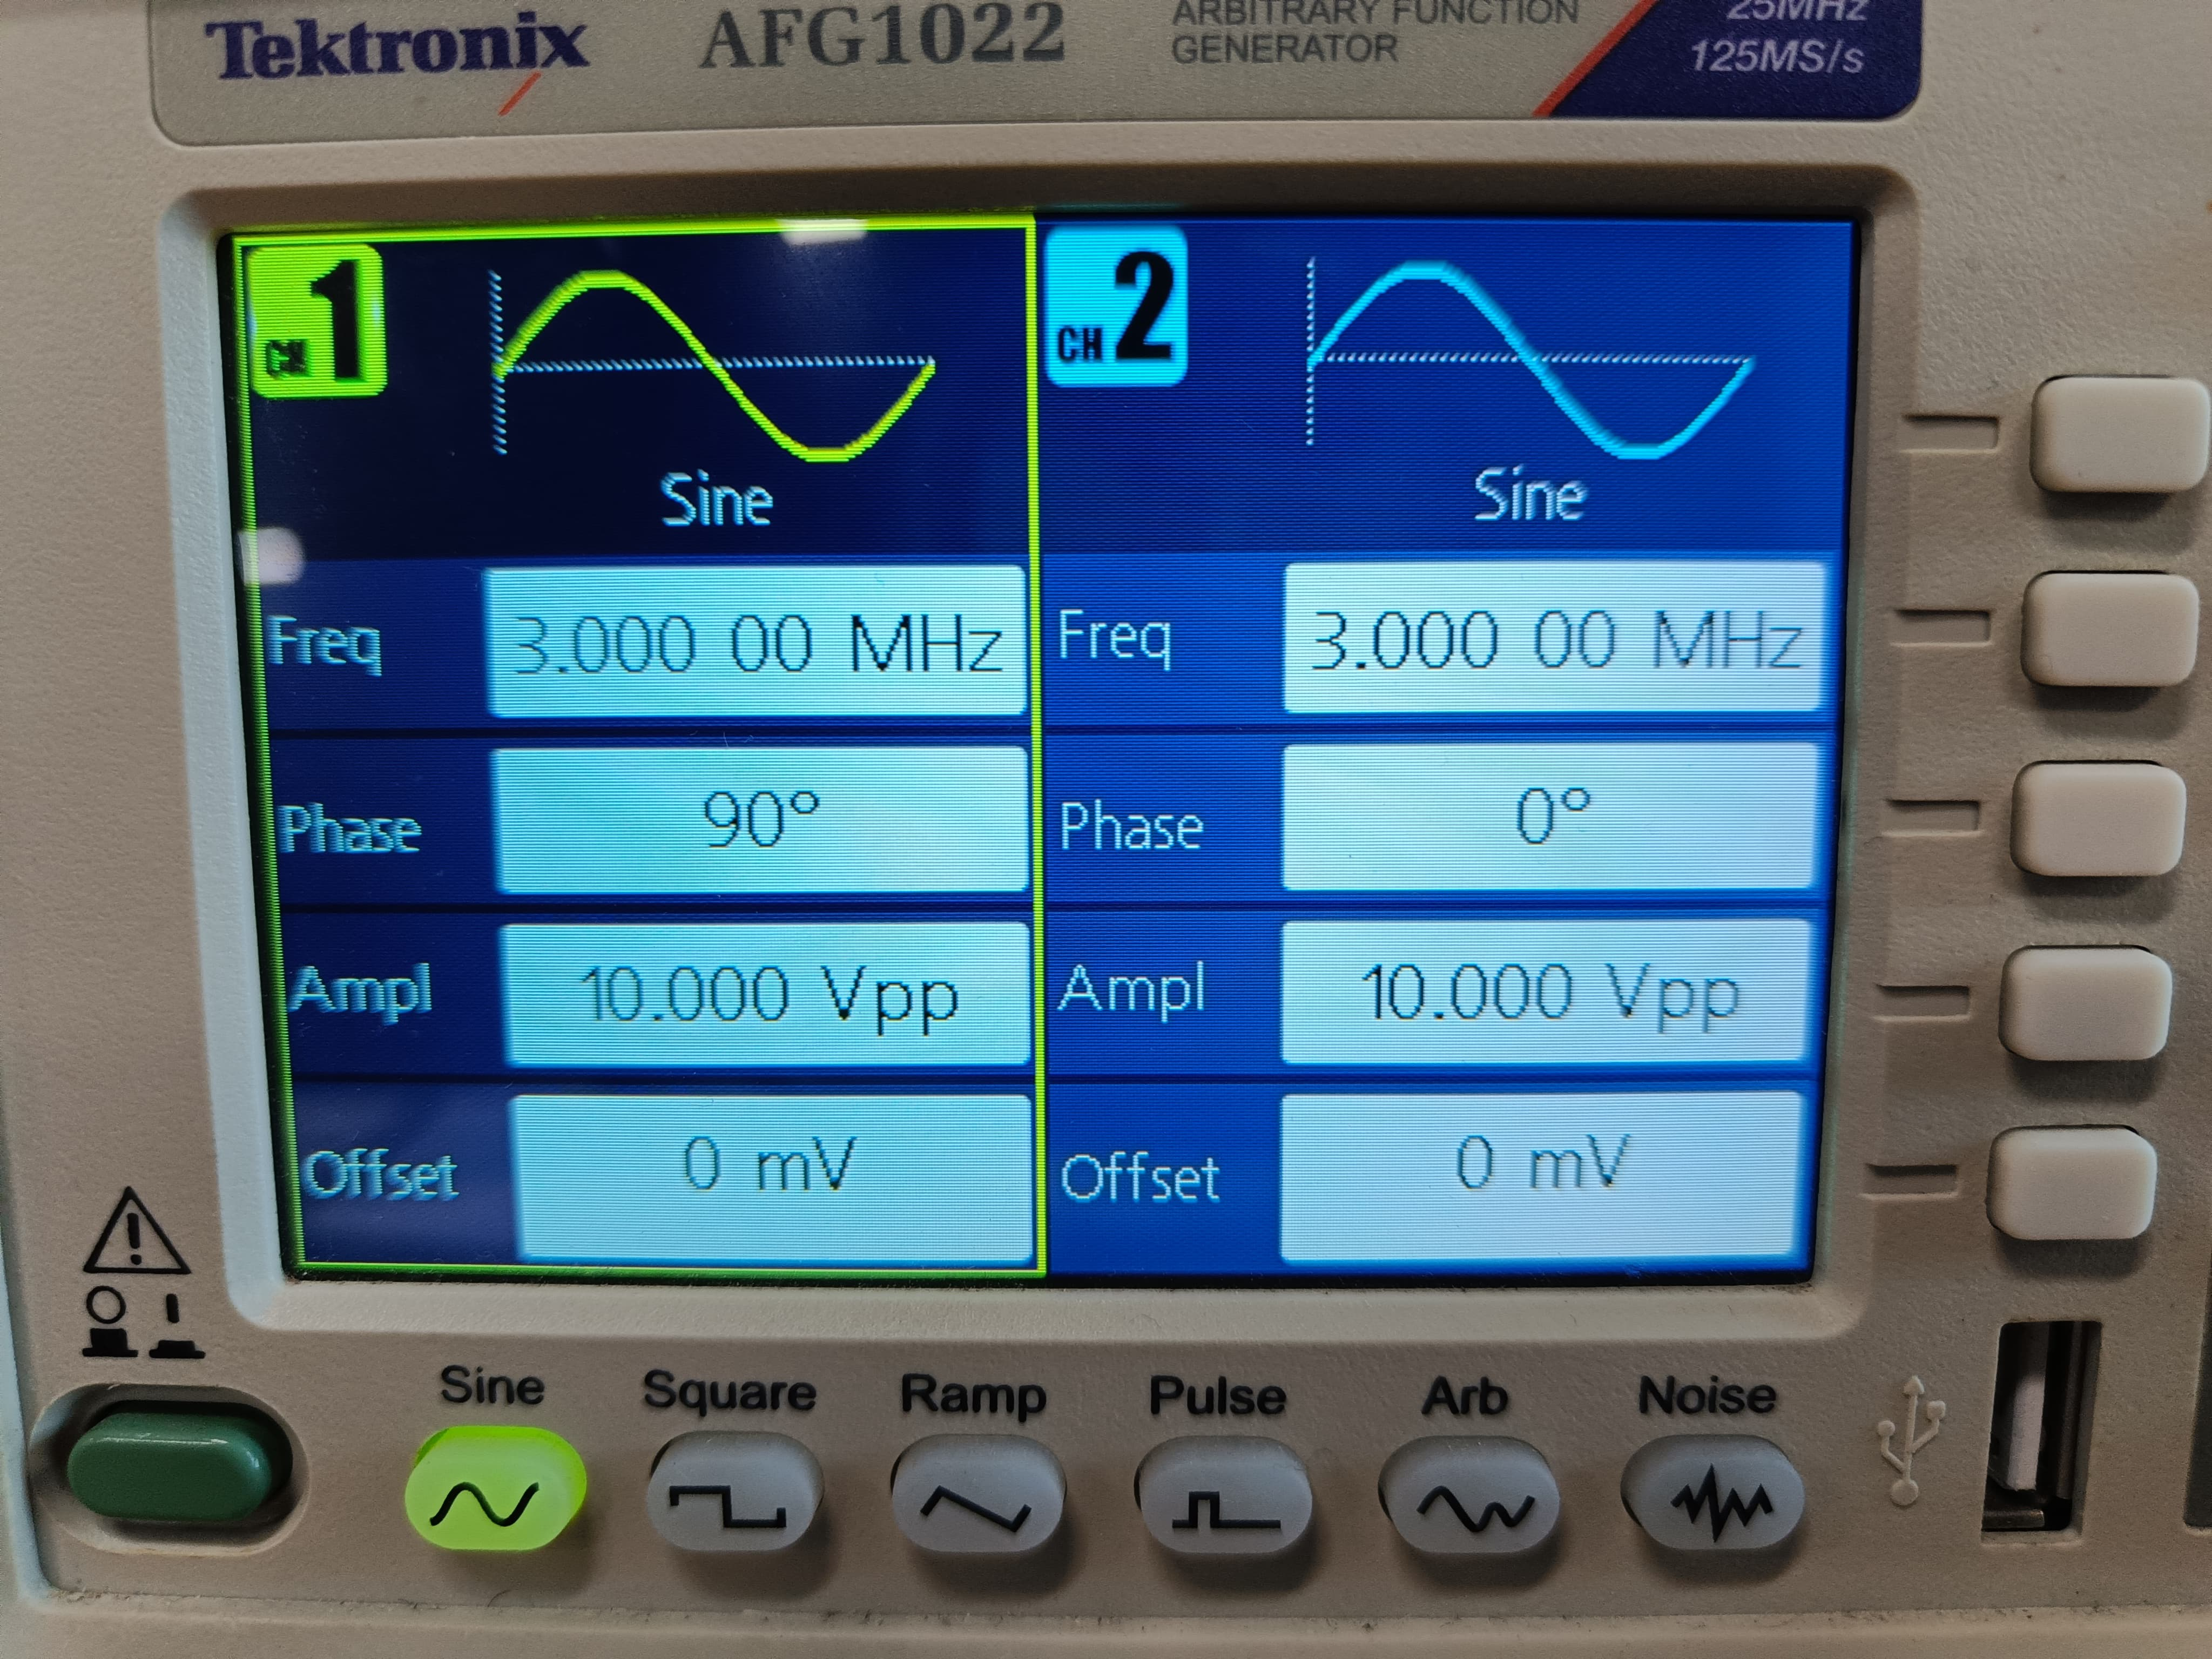
\includegraphics[width=0.7\columnwidth]{pics/WhatsApp Image 2025-01-23 at 13.22.01(1).jpeg}
        \caption{Input from function generator}
    \end{figure}
    \begin{figure}[H]
        \centering
        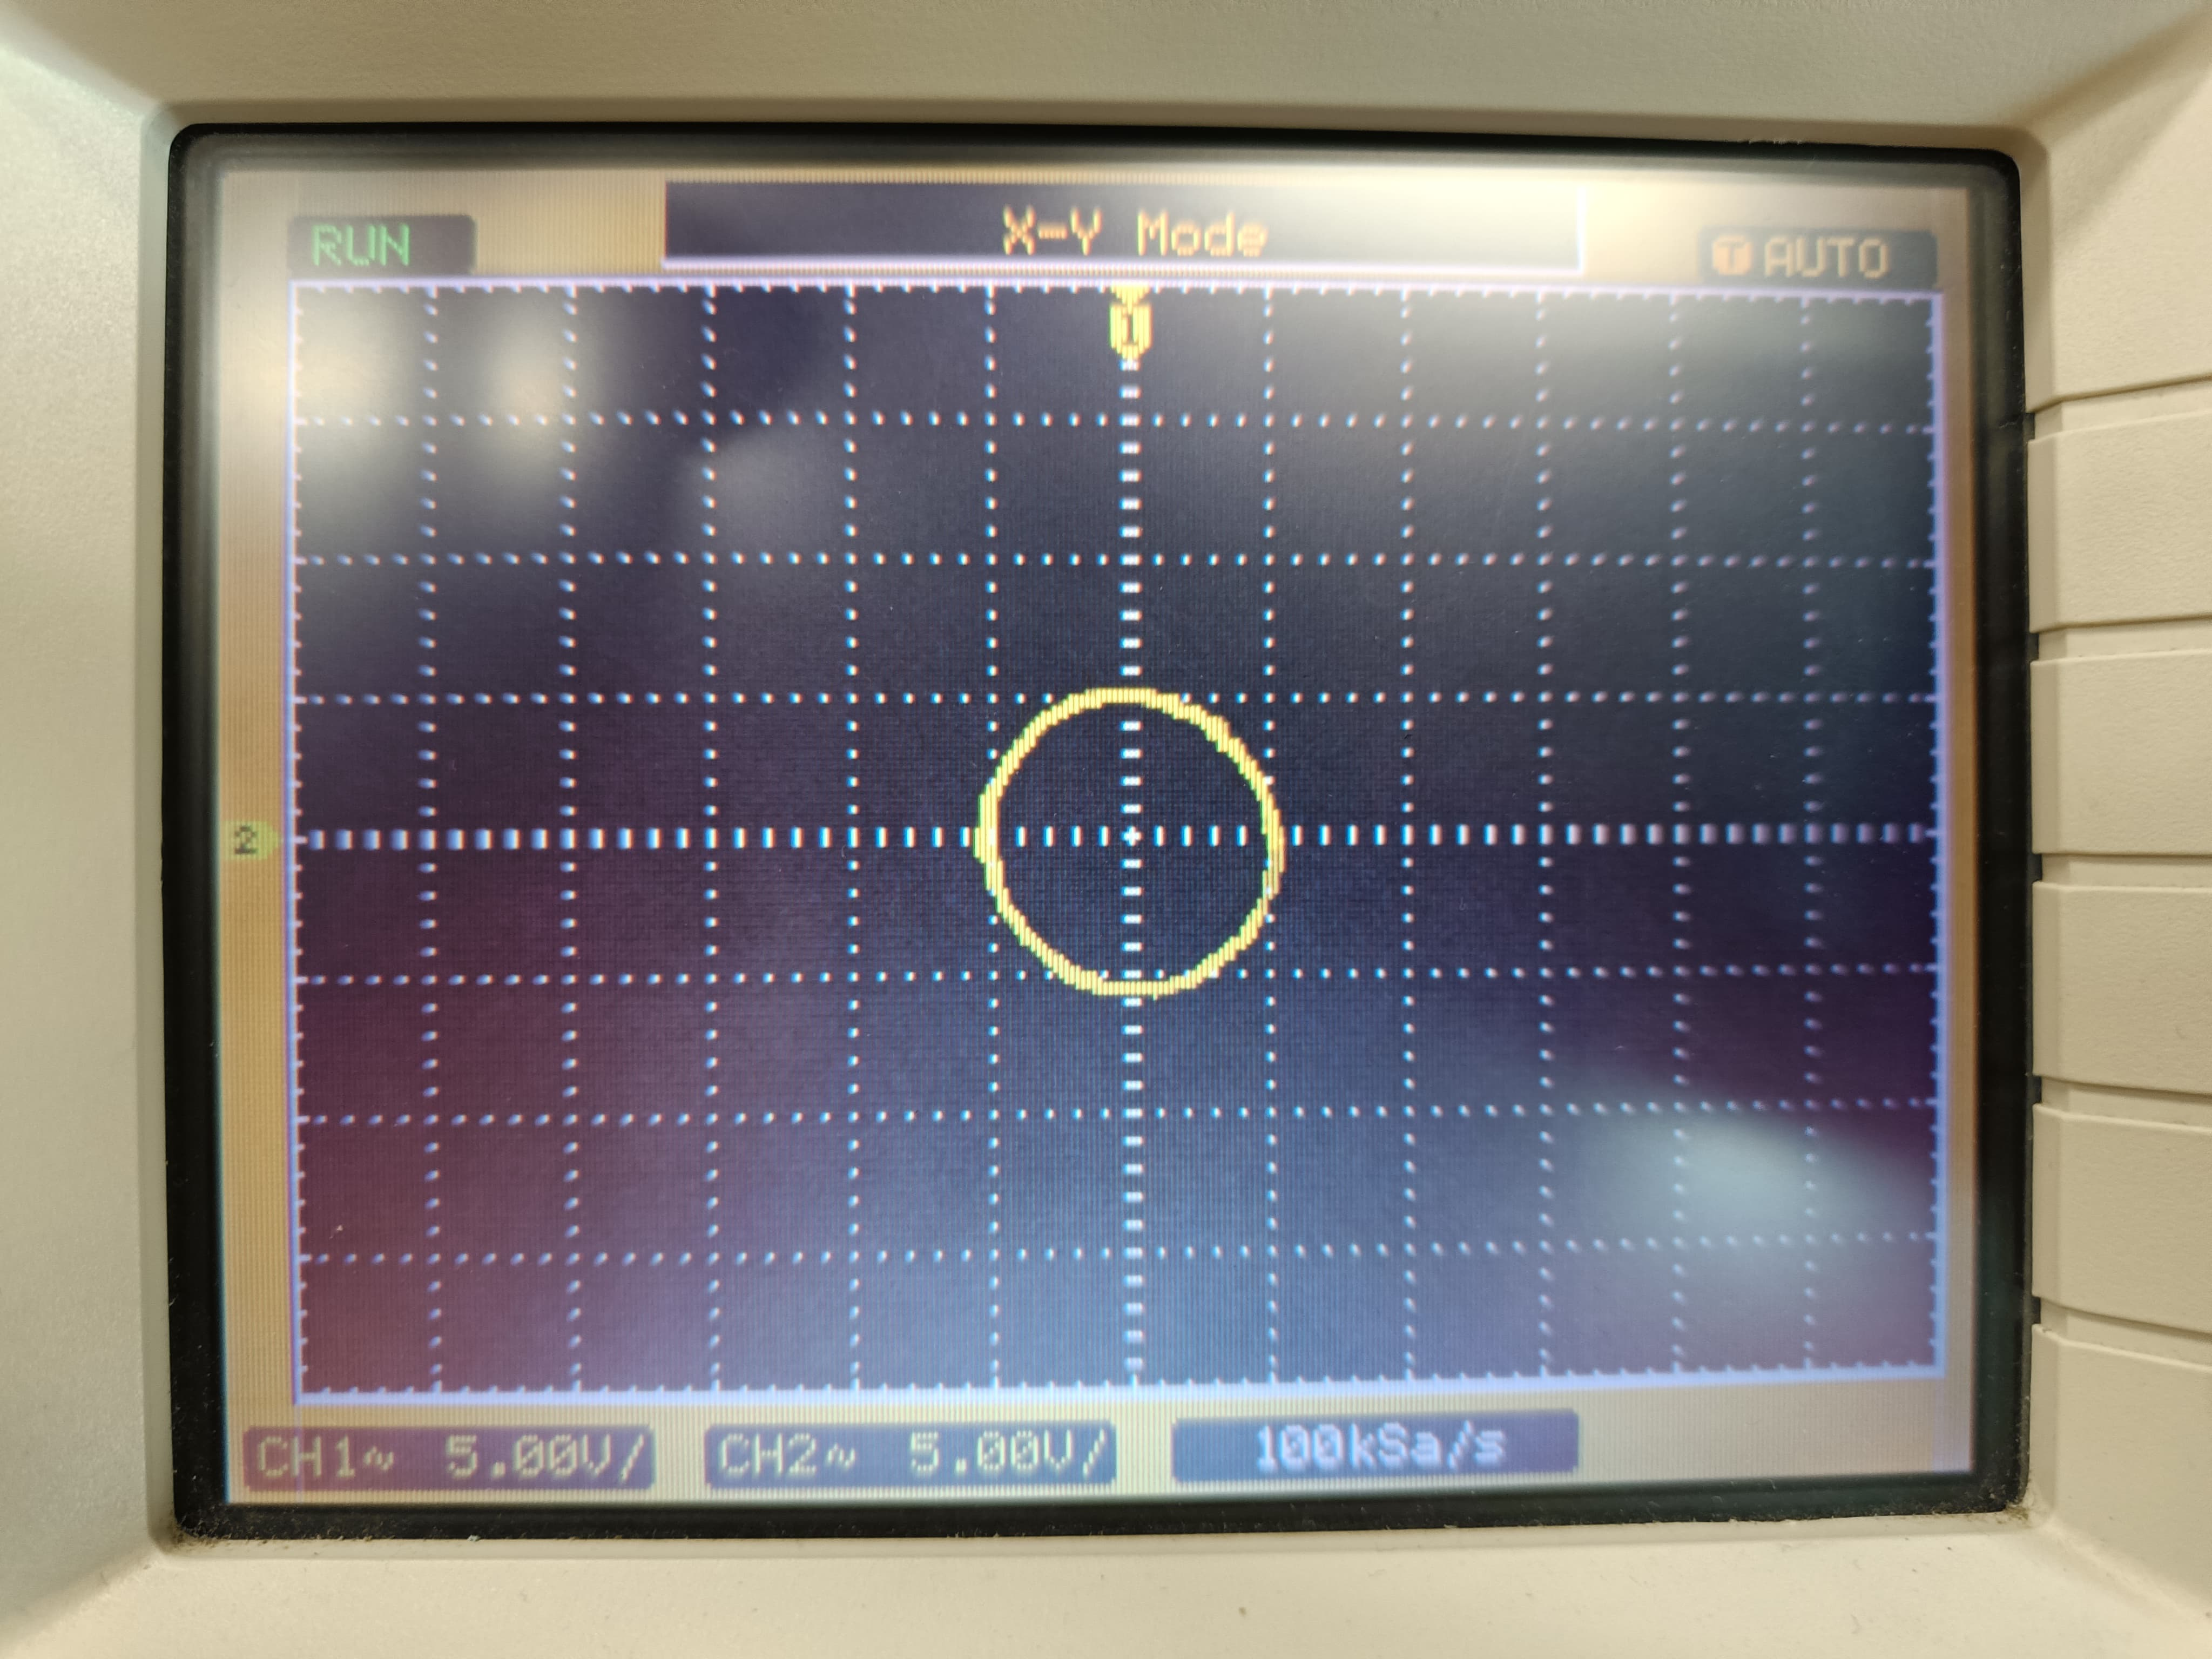
\includegraphics[width=0.7\columnwidth]{pics/WhatsApp Image 2025-01-23 at 13.22.01.jpeg}
        \caption{Output on CRO}
    \end{figure}
    \begin{figure}[H]
        \centering
        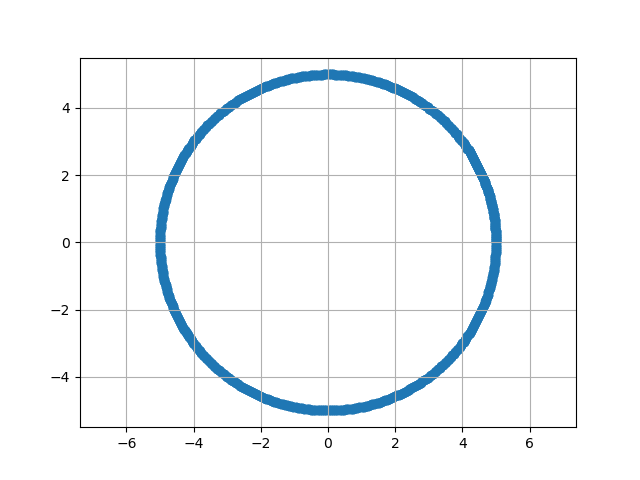
\includegraphics[width=0.7\columnwidth]{figs/fig2.png}
        \caption{Theoretical Plot}
    \end{figure}
    %3
    \item \begin{align}
        x = 5\sin\brak{\frac{2\pi}{3}t+\frac{\pi}{2}}, y = 5\sin\brak{\frac{2\pi}{6}t}
    \end{align}
    \begin{figure}[H]
        \centering
        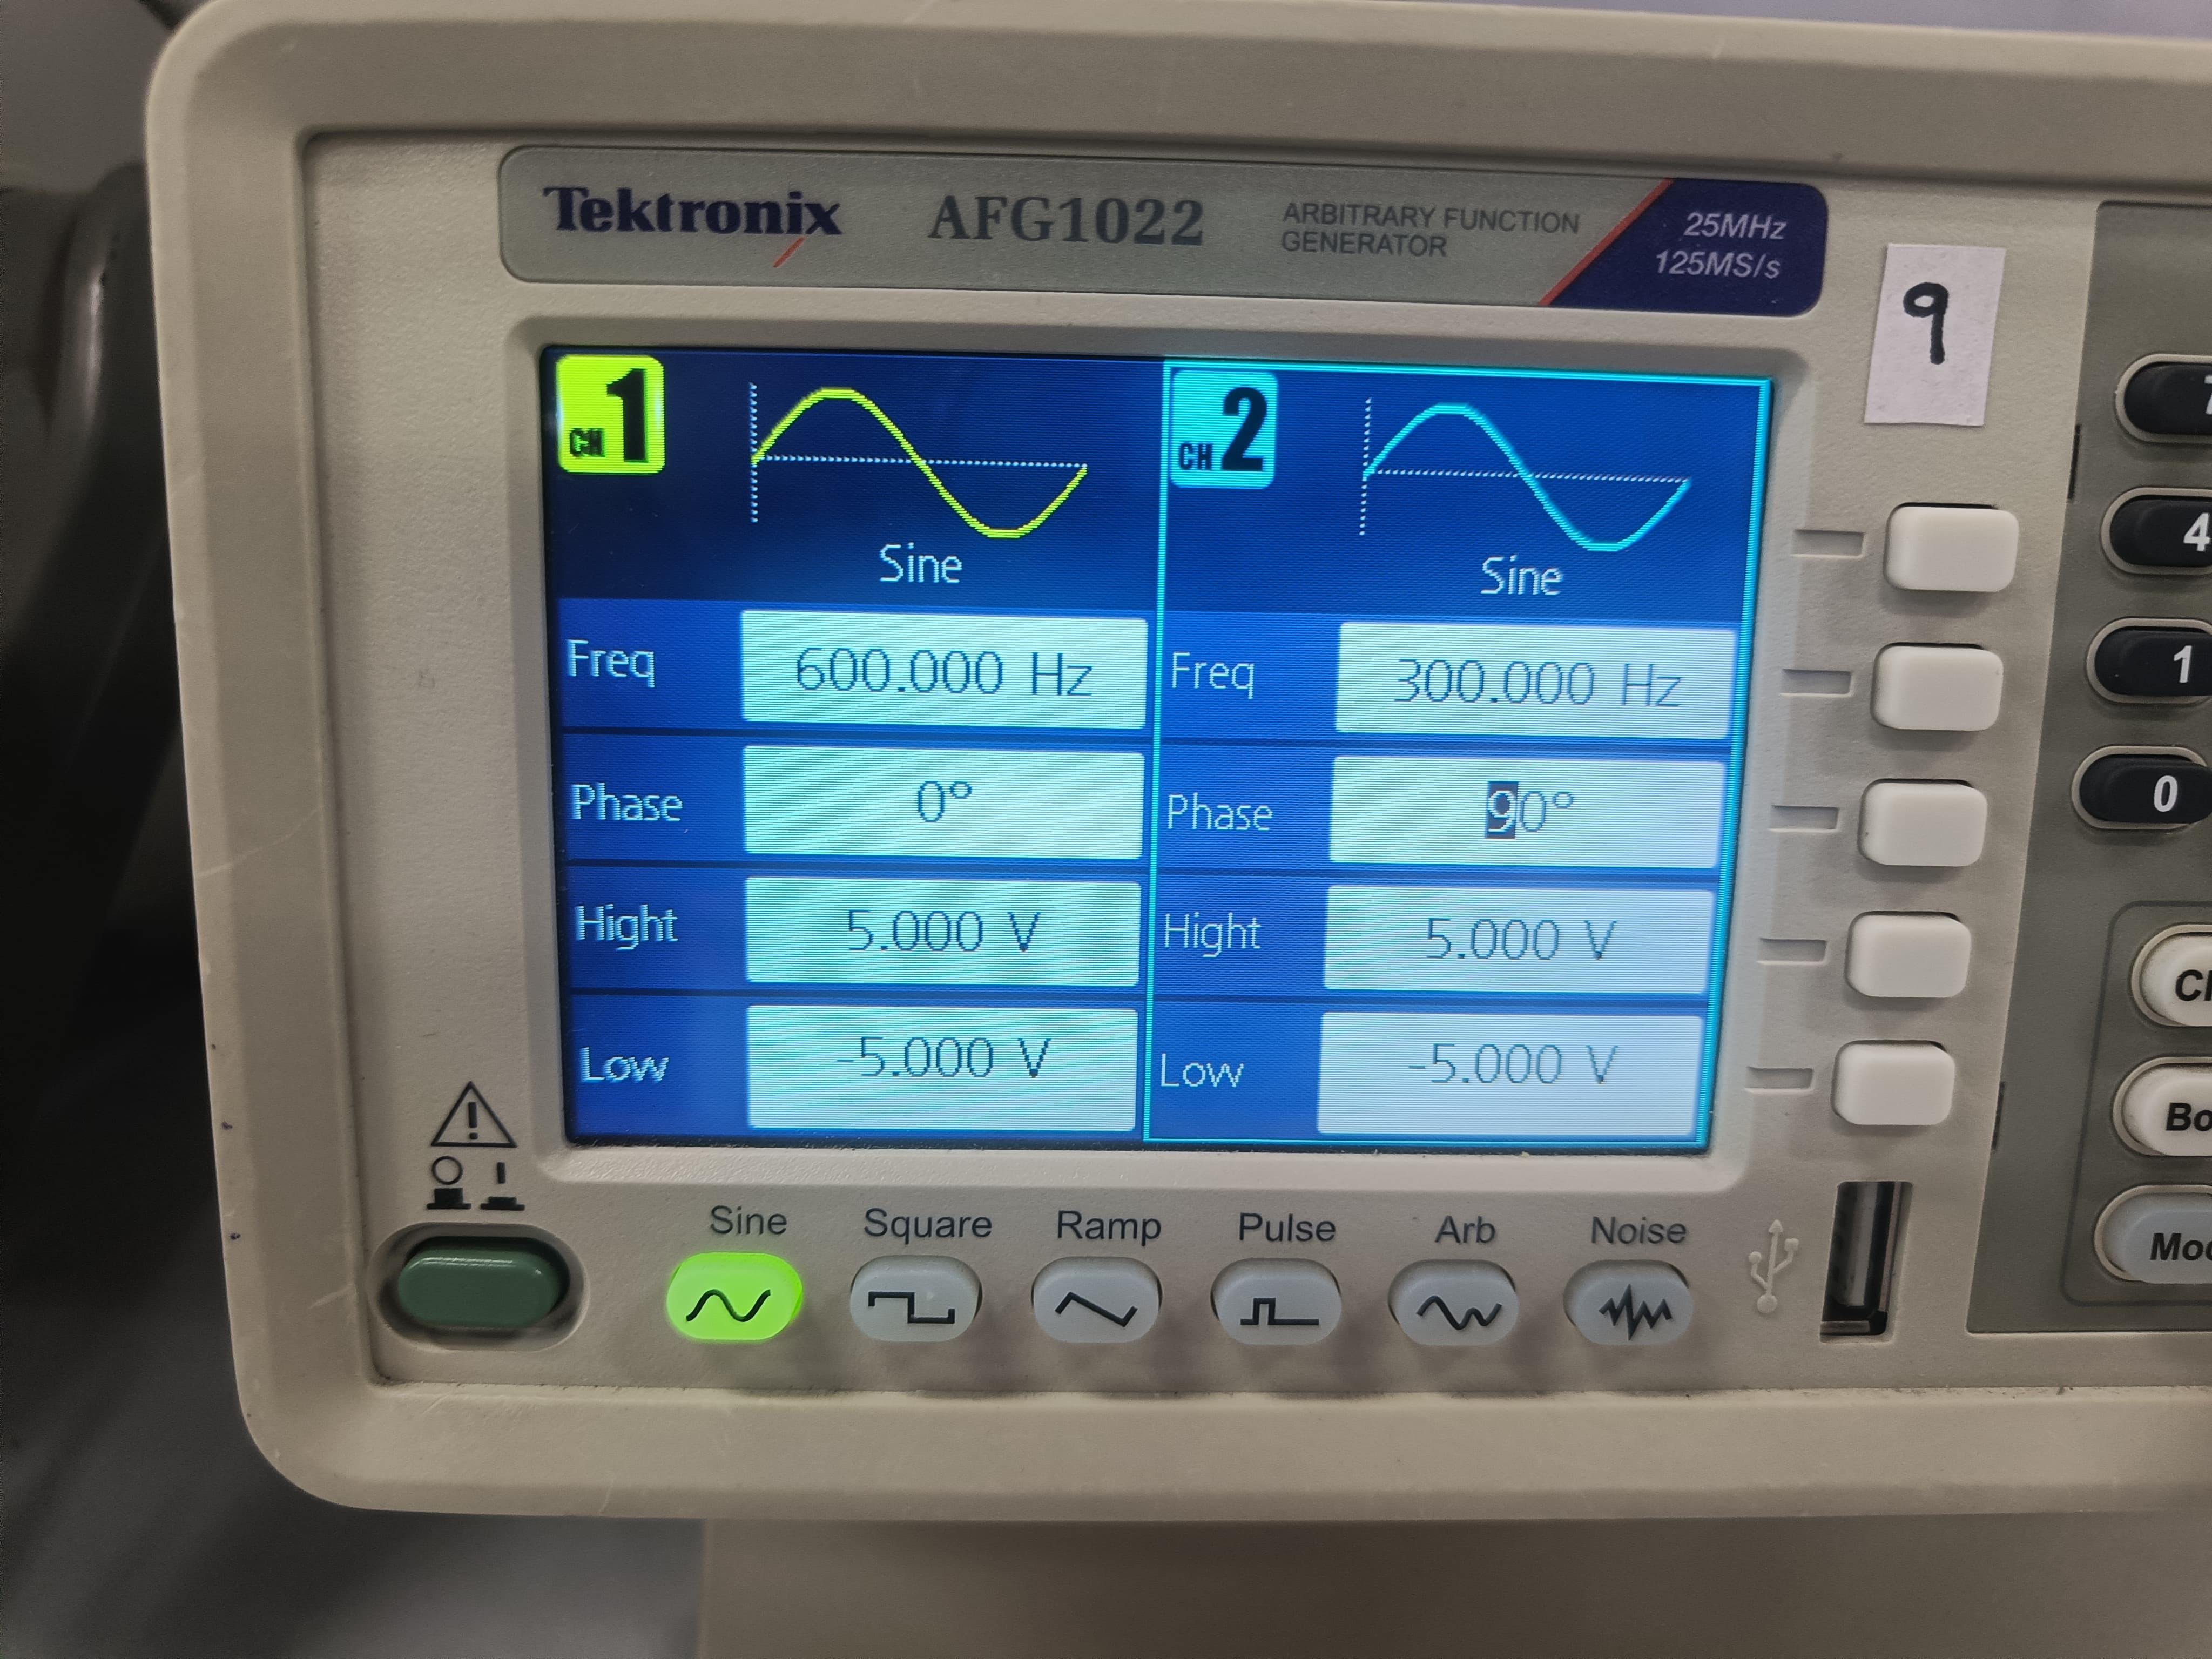
\includegraphics[width=0.7\columnwidth]{pics/WhatsApp Image 2025-01-24 at 11.02.17.jpeg}
        \caption{Input from function generator}
    \end{figure}
    \begin{figure}[H]
        \centering
        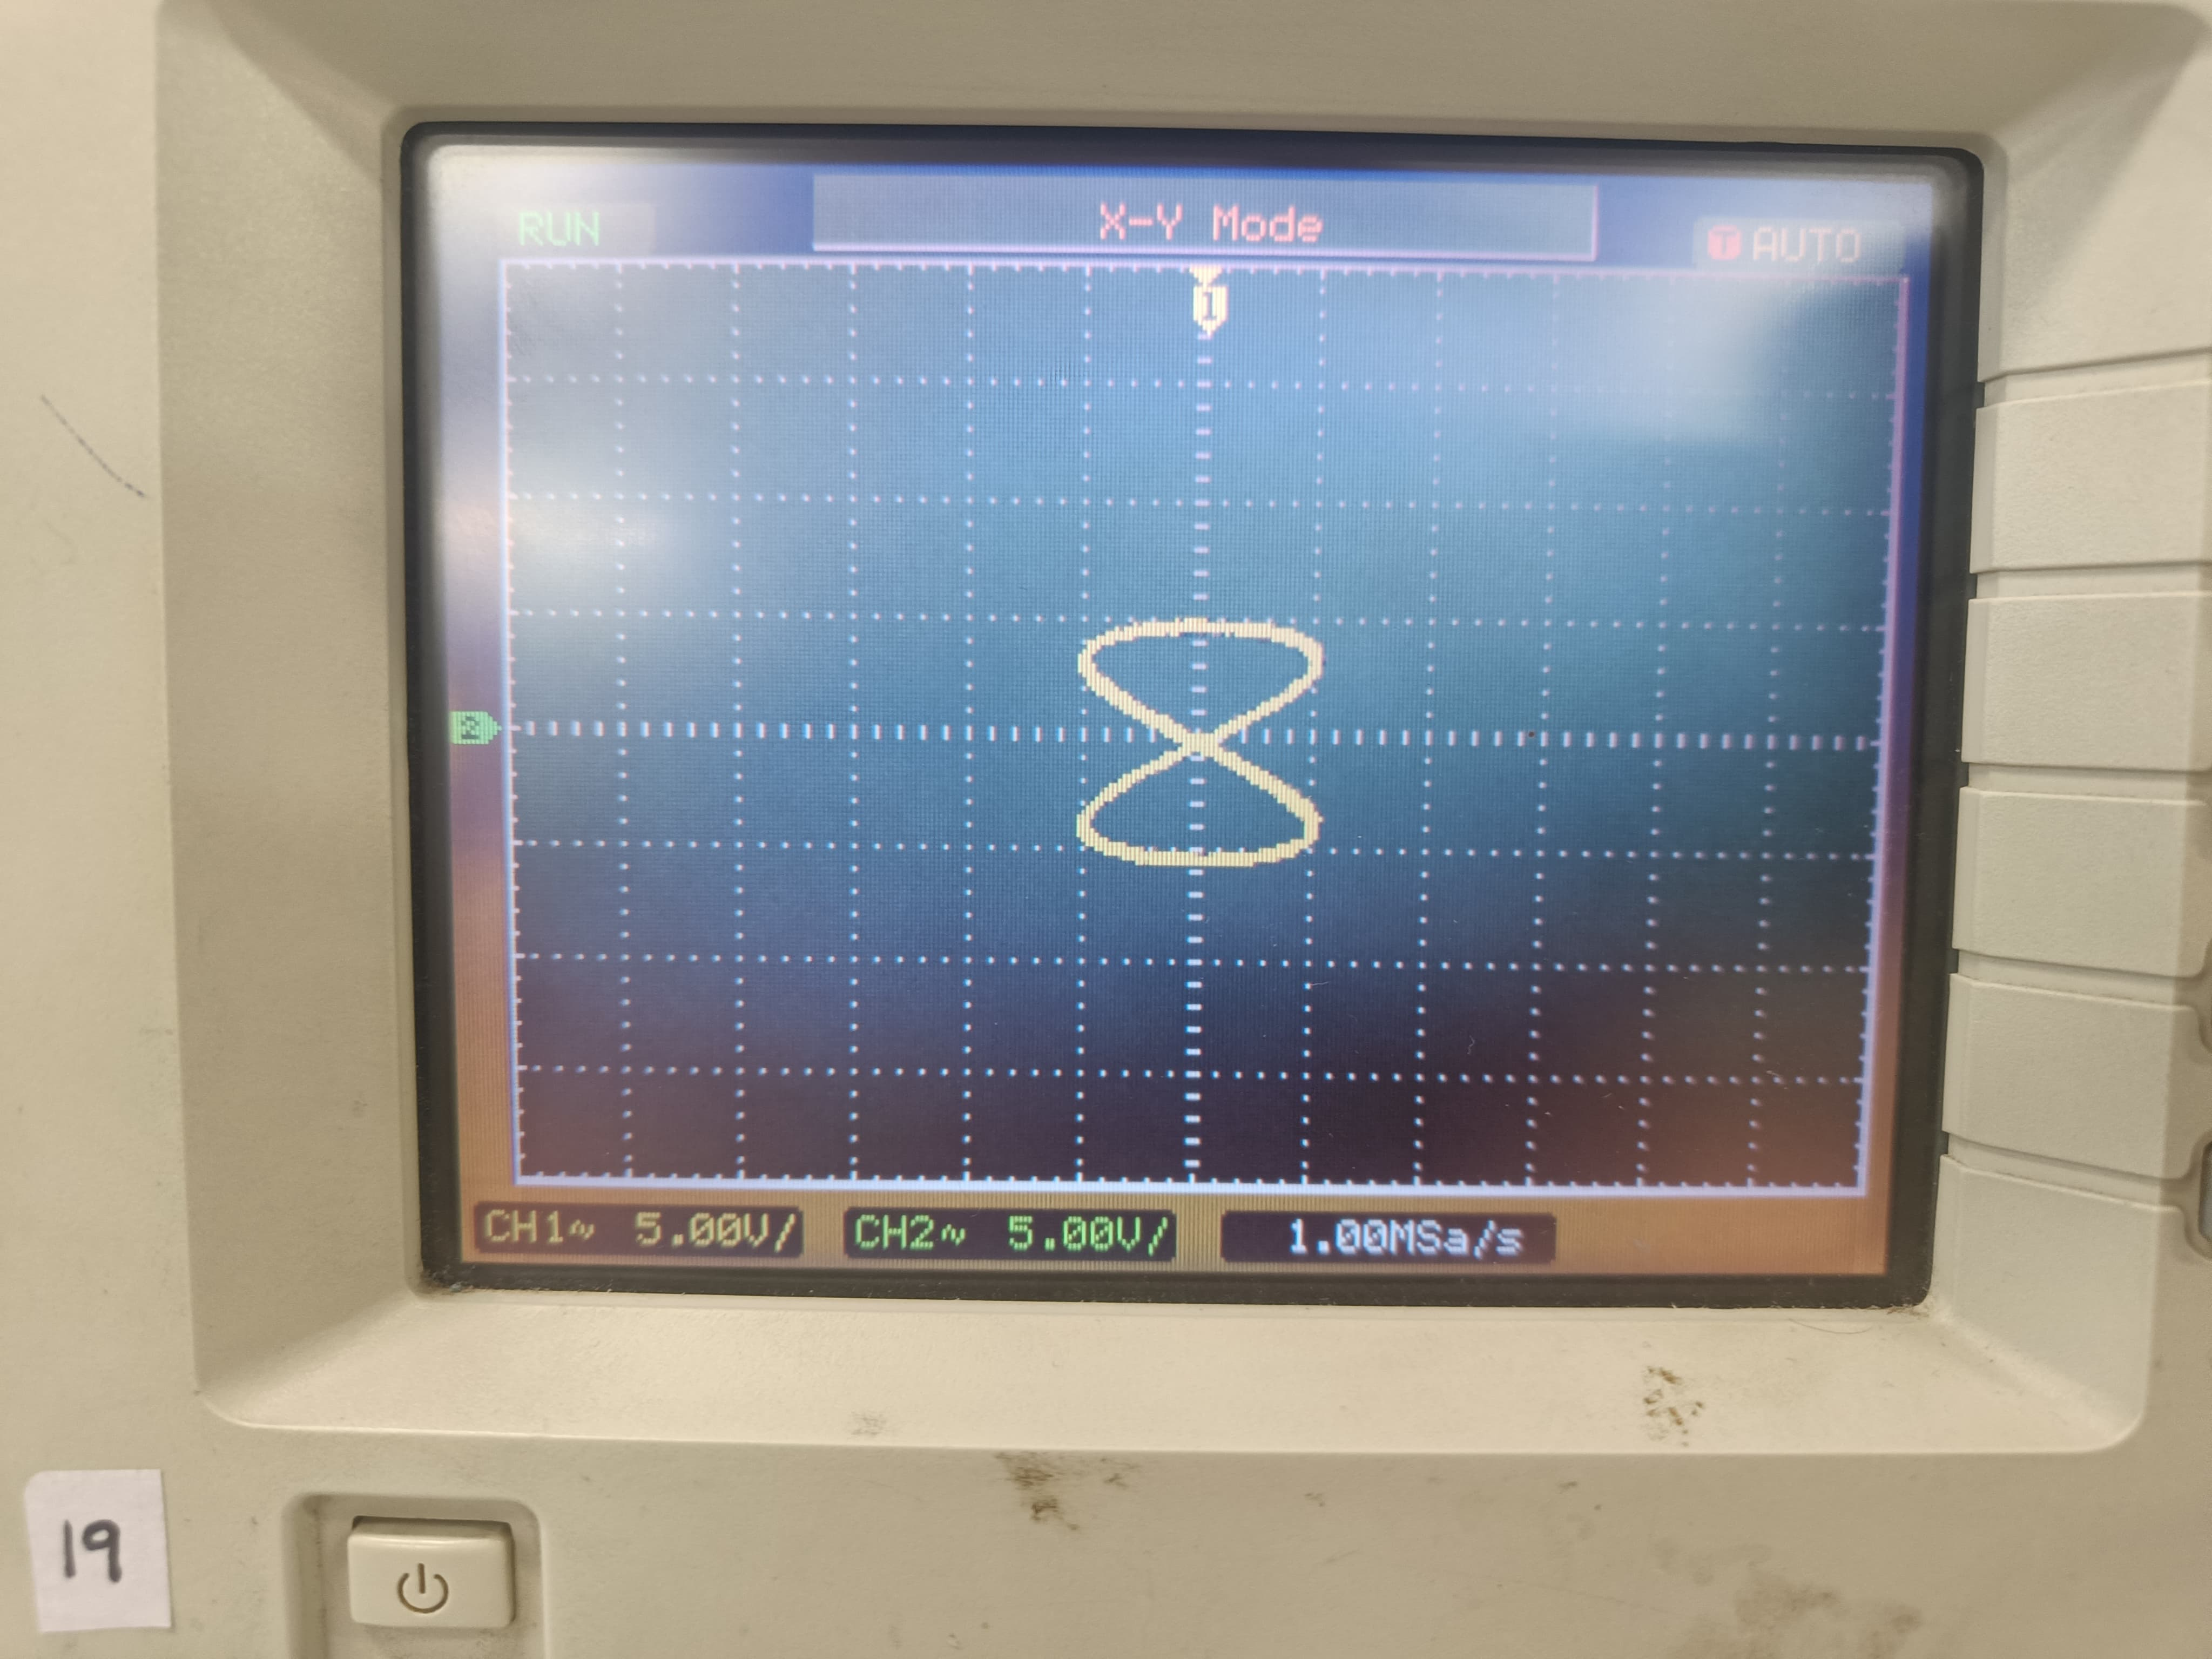
\includegraphics[width=0.7\columnwidth]{pics/WhatsApp Image 2025-01-24 at 11.02.16(3).jpeg}
        \caption{Output on CRO}
    \end{figure}
    \begin{figure}[H]
        \centering
        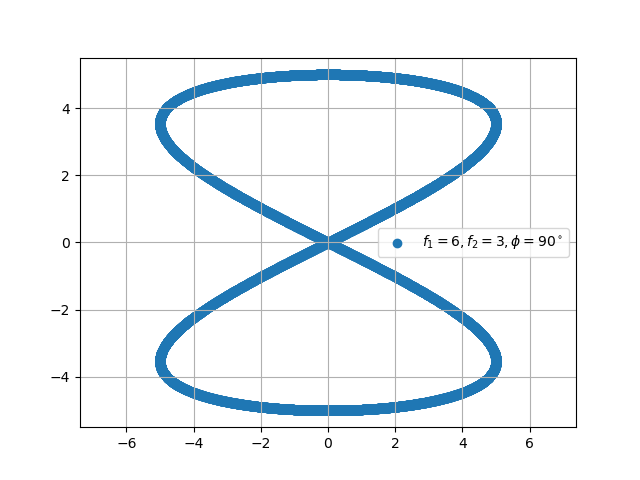
\includegraphics[width=0.7\columnwidth]{figs/fig4.png}
        \caption{Theoretical Plot}
    \end{figure}
    %4
    \item \begin{align}
        x = 5\sin\brak{\frac{2\pi}{4}t+\frac{\pi}{4}},\,y = 5\sin\brak{\frac{2\pi}{3}t}
    \end{align}
    \begin{figure}[H]
        \centering
        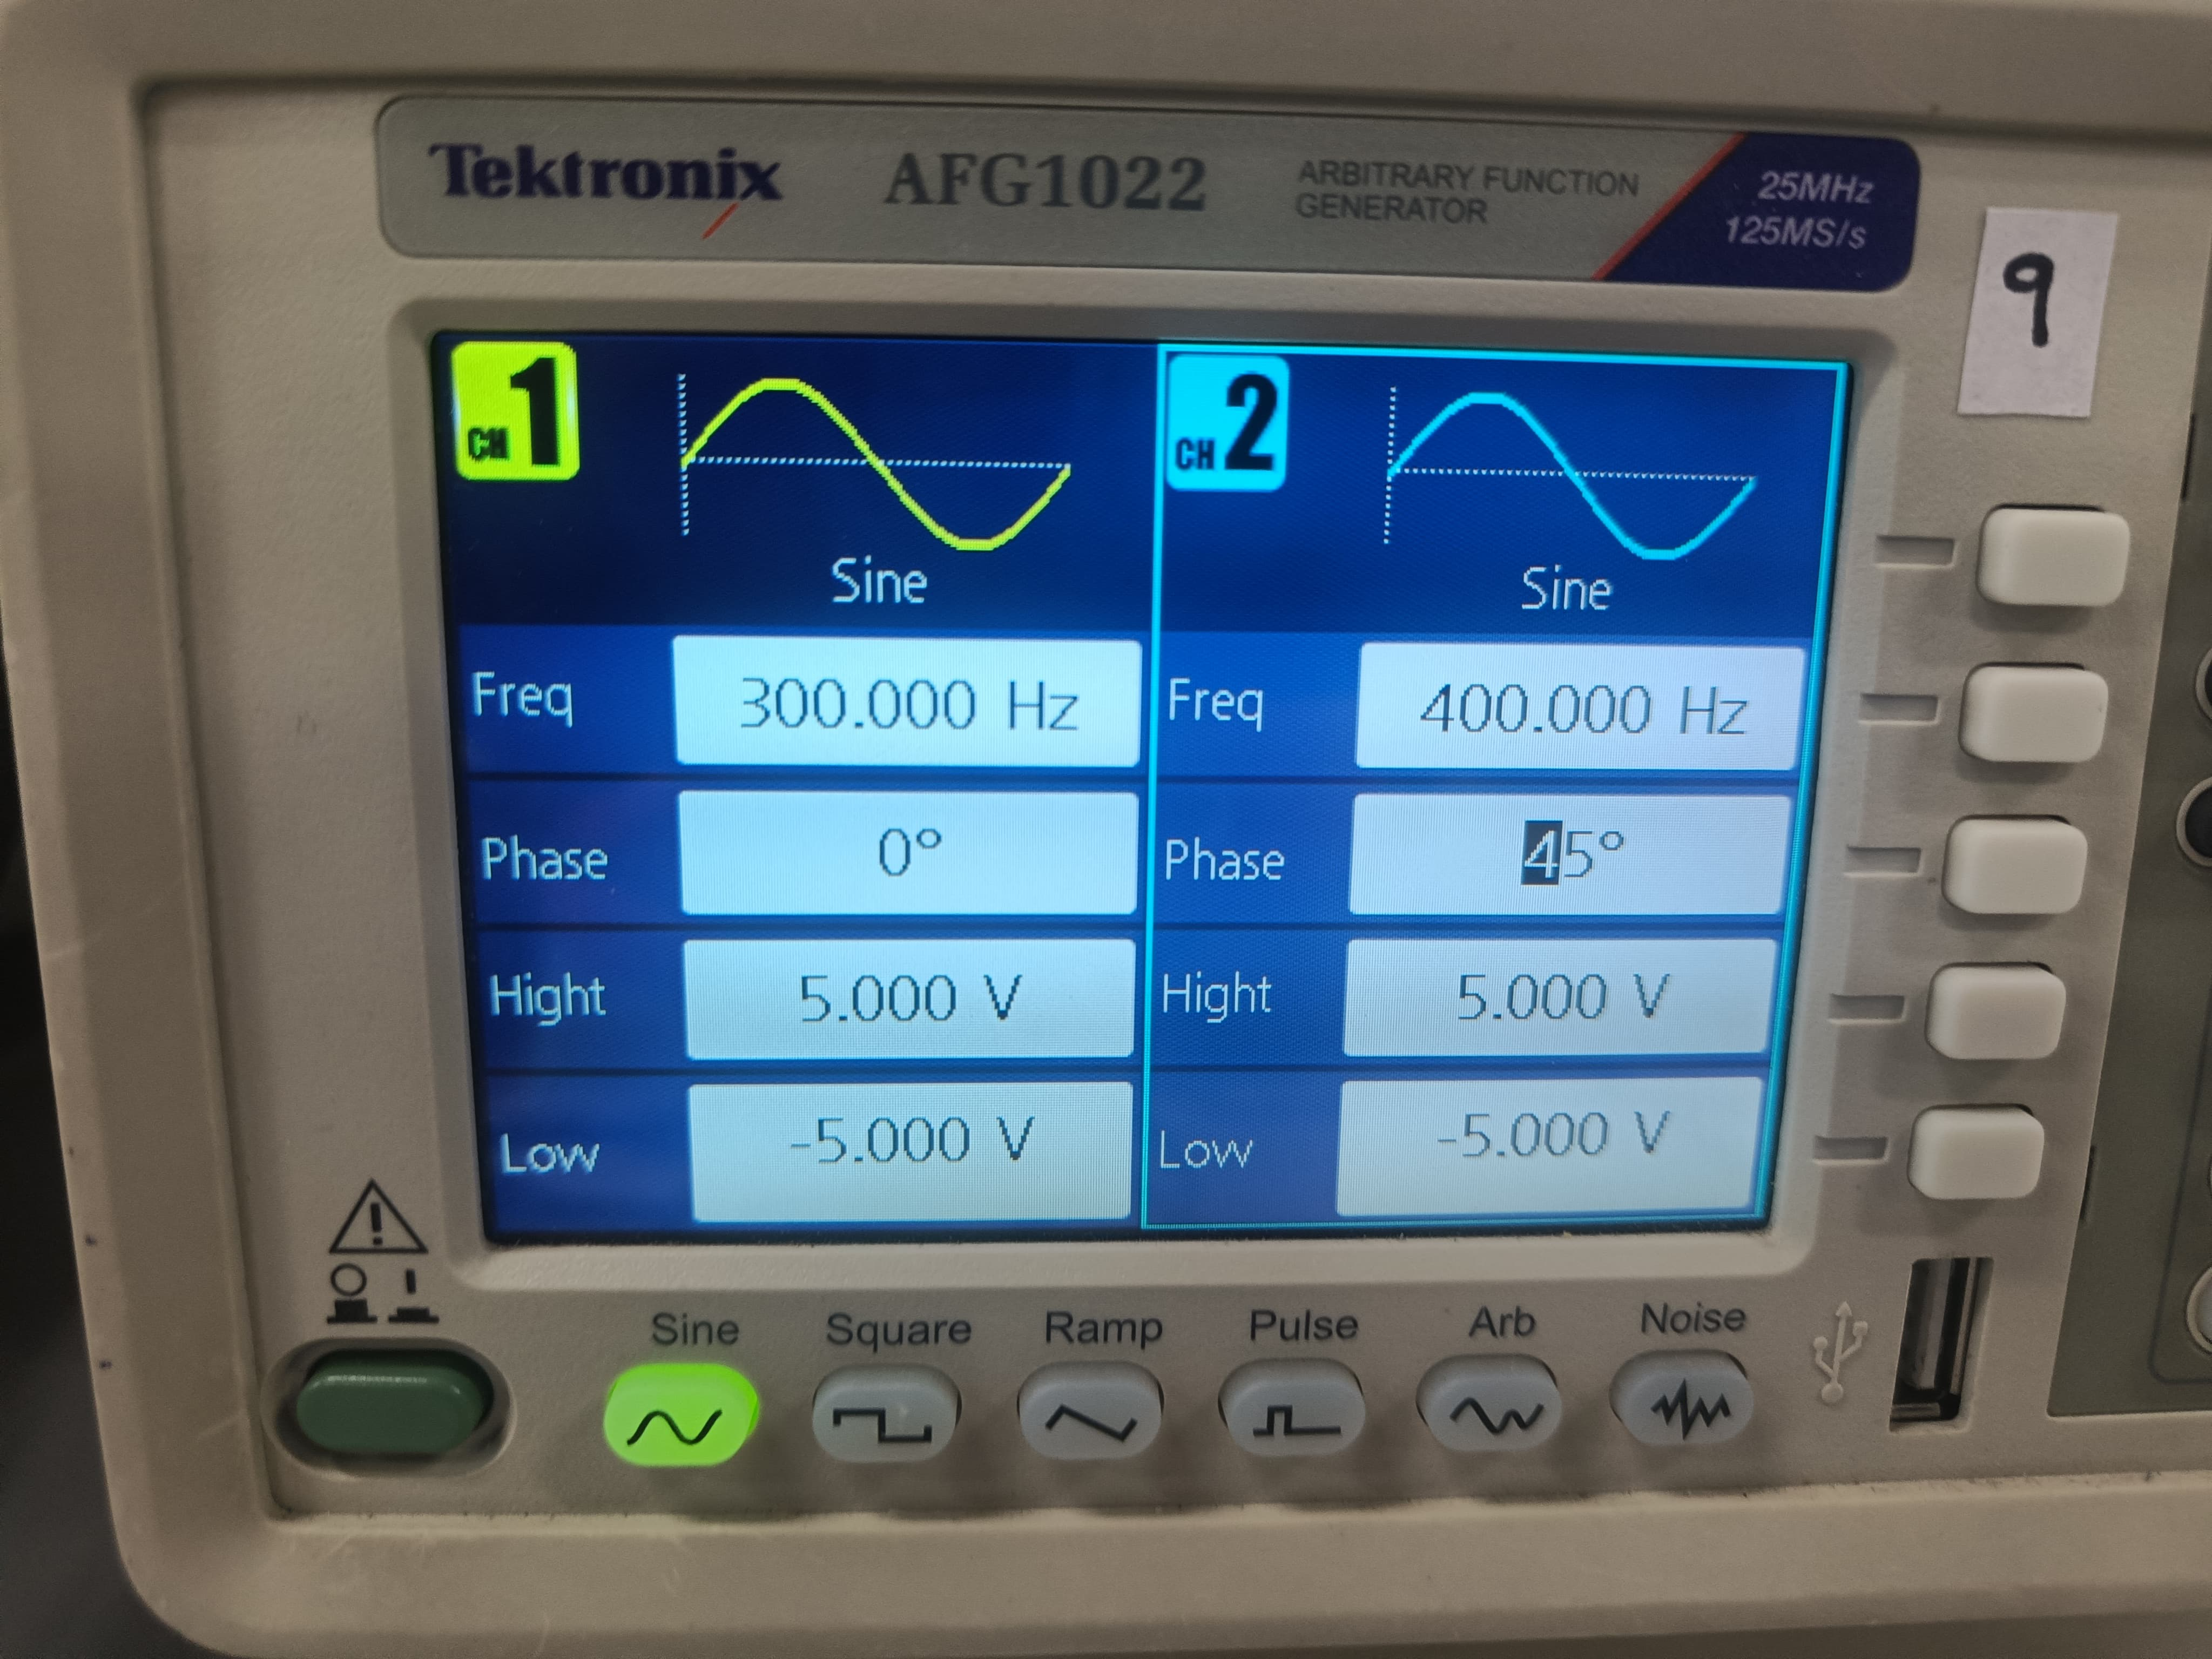
\includegraphics[width=0.7\columnwidth]{pics/WhatsApp Image 2025-01-24 at 11.02.16(2).jpeg}
        \caption{Input from function generator}
    \end{figure}
    \begin{figure}[H]
        \centering
        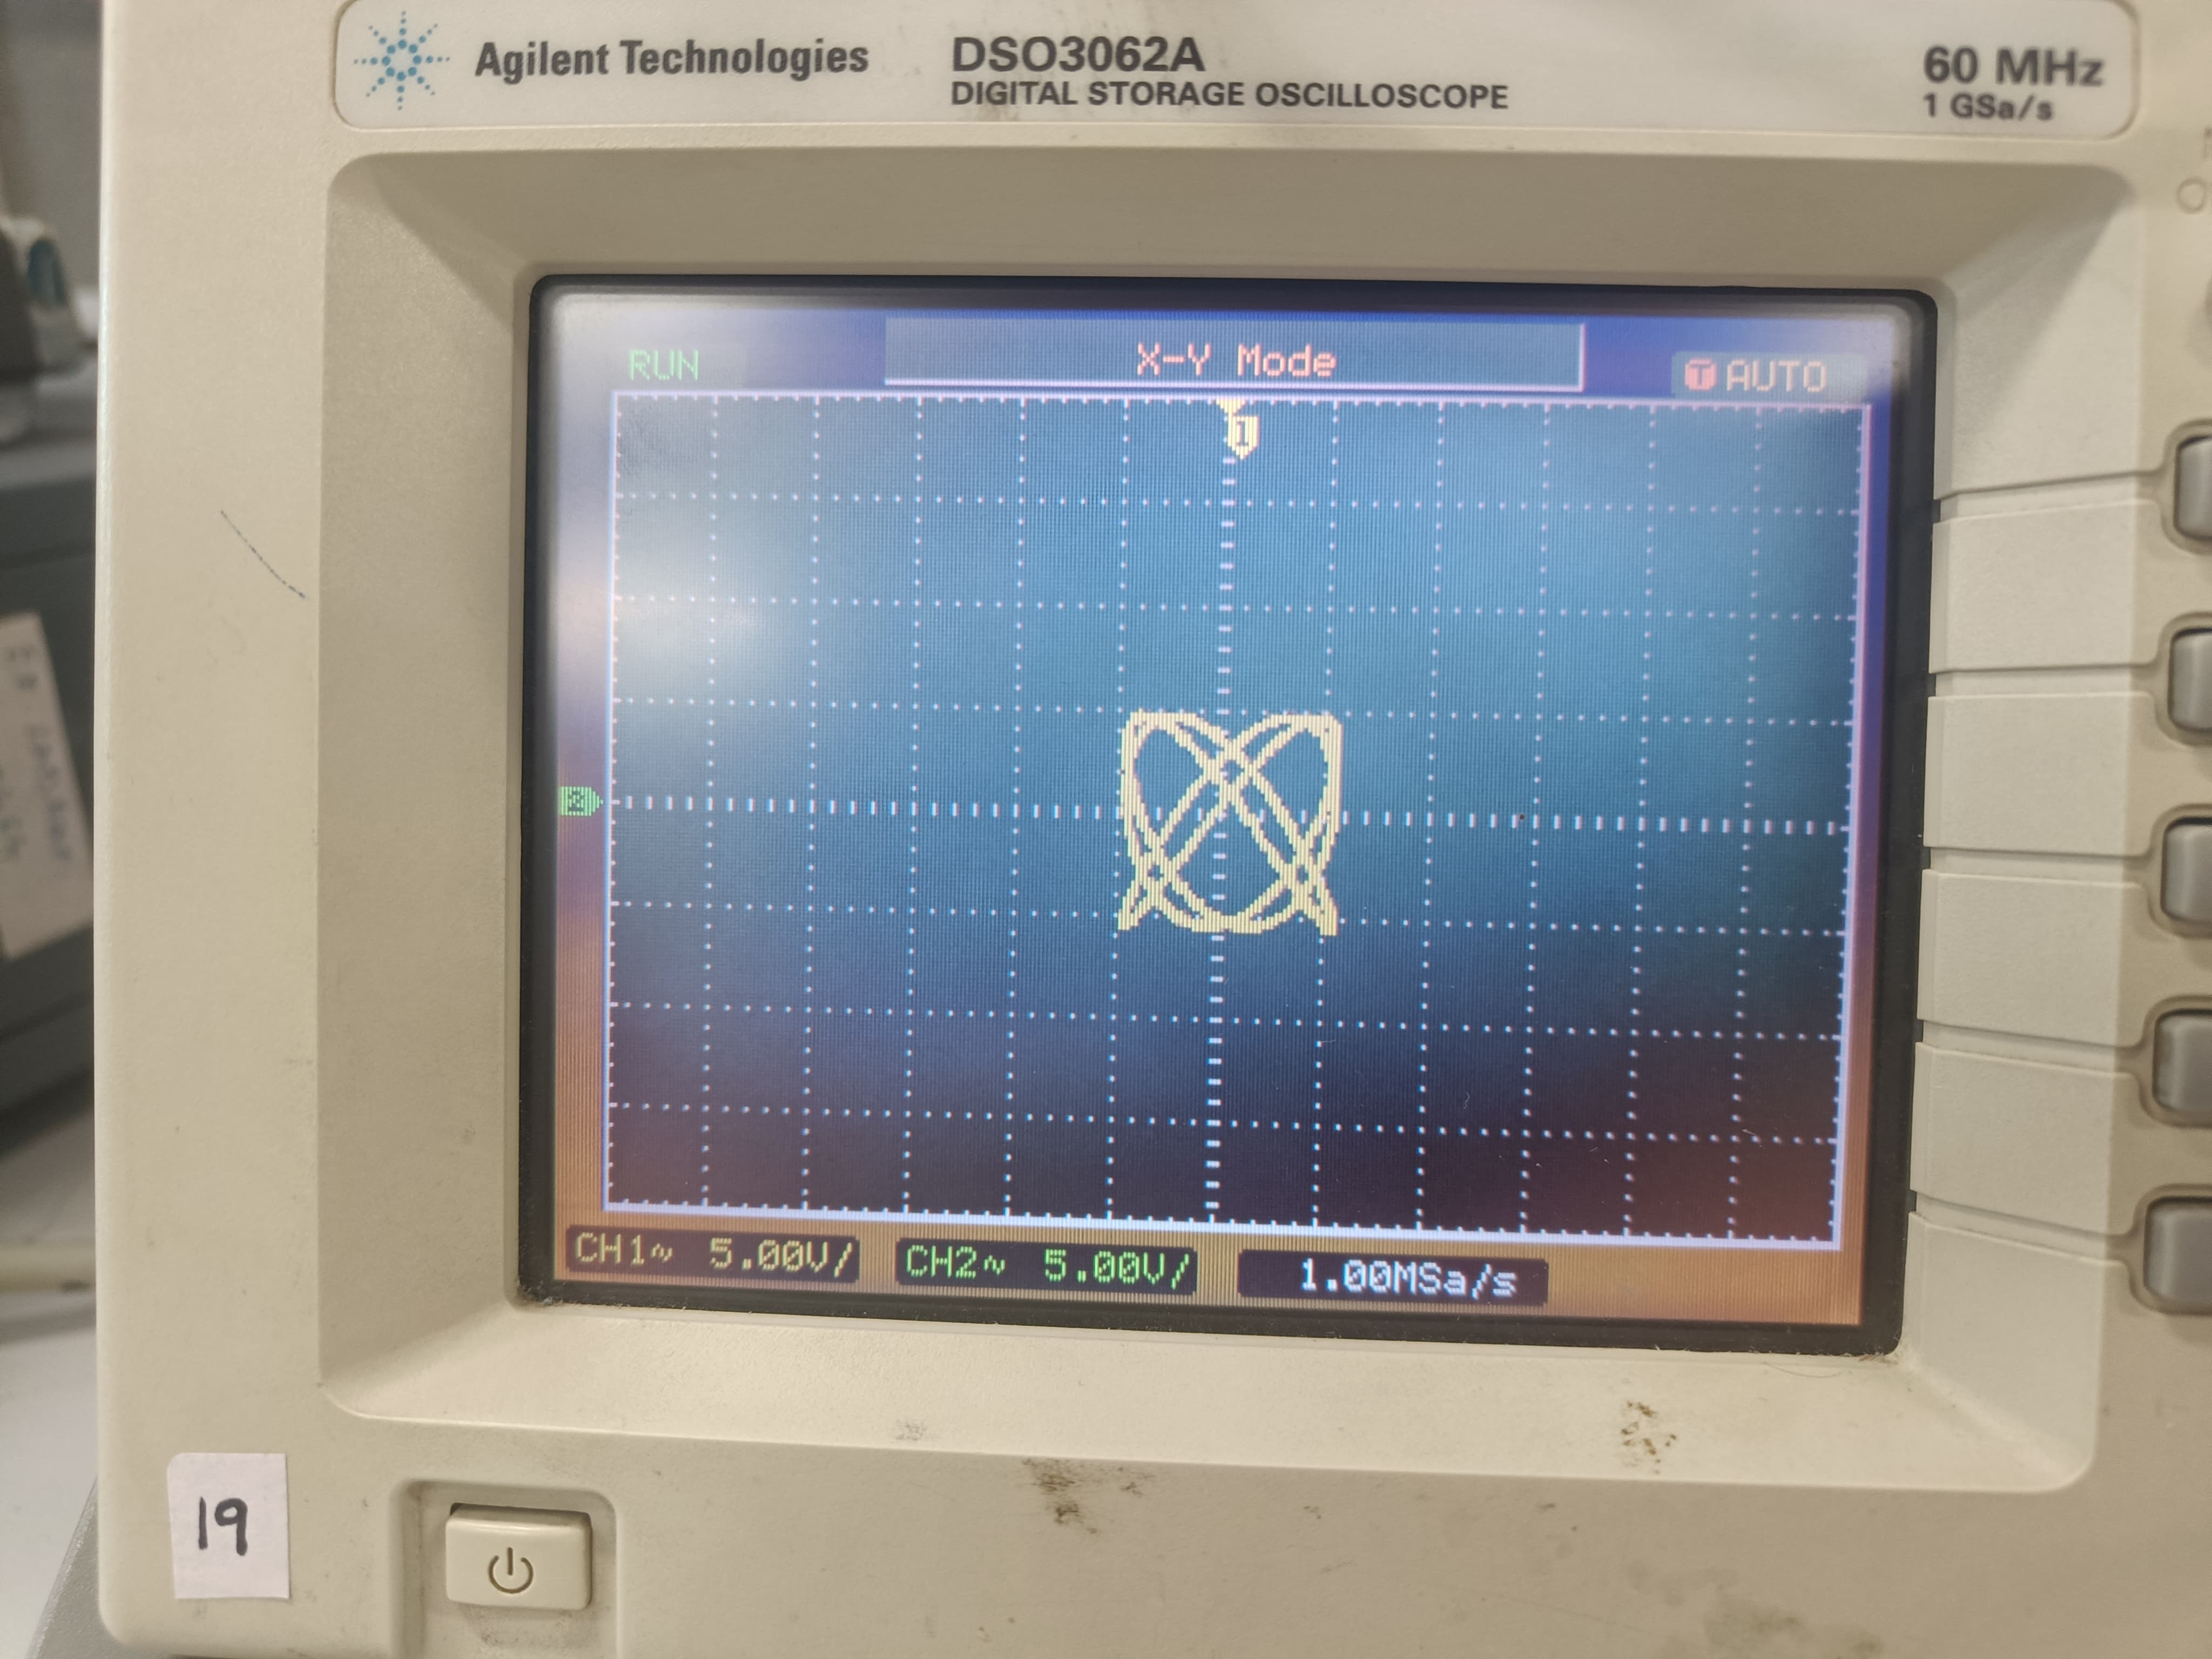
\includegraphics[width=0.7\columnwidth]{pics/WhatsApp Image 2025-01-24 at 11.02.16(1).jpeg}
        \caption{Output on CRO}
    \end{figure}
    \begin{figure}[H]
        \centering
        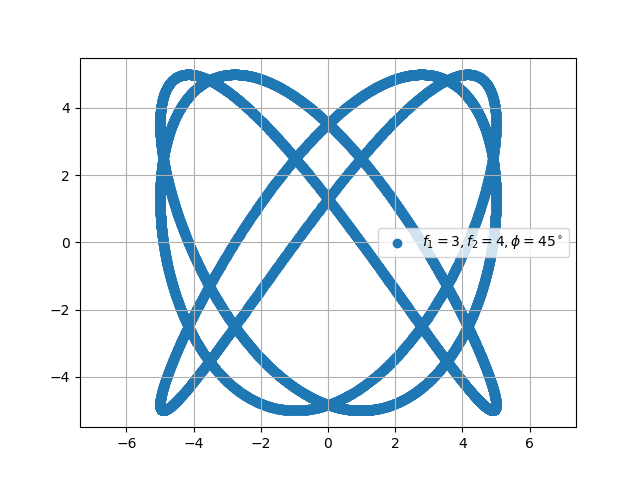
\includegraphics[width=0.7\columnwidth]{figs/fig3.png}
        \caption{Theoretical Plot}
    \end{figure}
    %5
    \item \begin{align}
        x = 5\sin\brak{\frac{2\pi}{3}t},\,y = 5\sin\brak{{2\pi}t}
    \end{align}
    \begin{figure}[H]
        \centering
        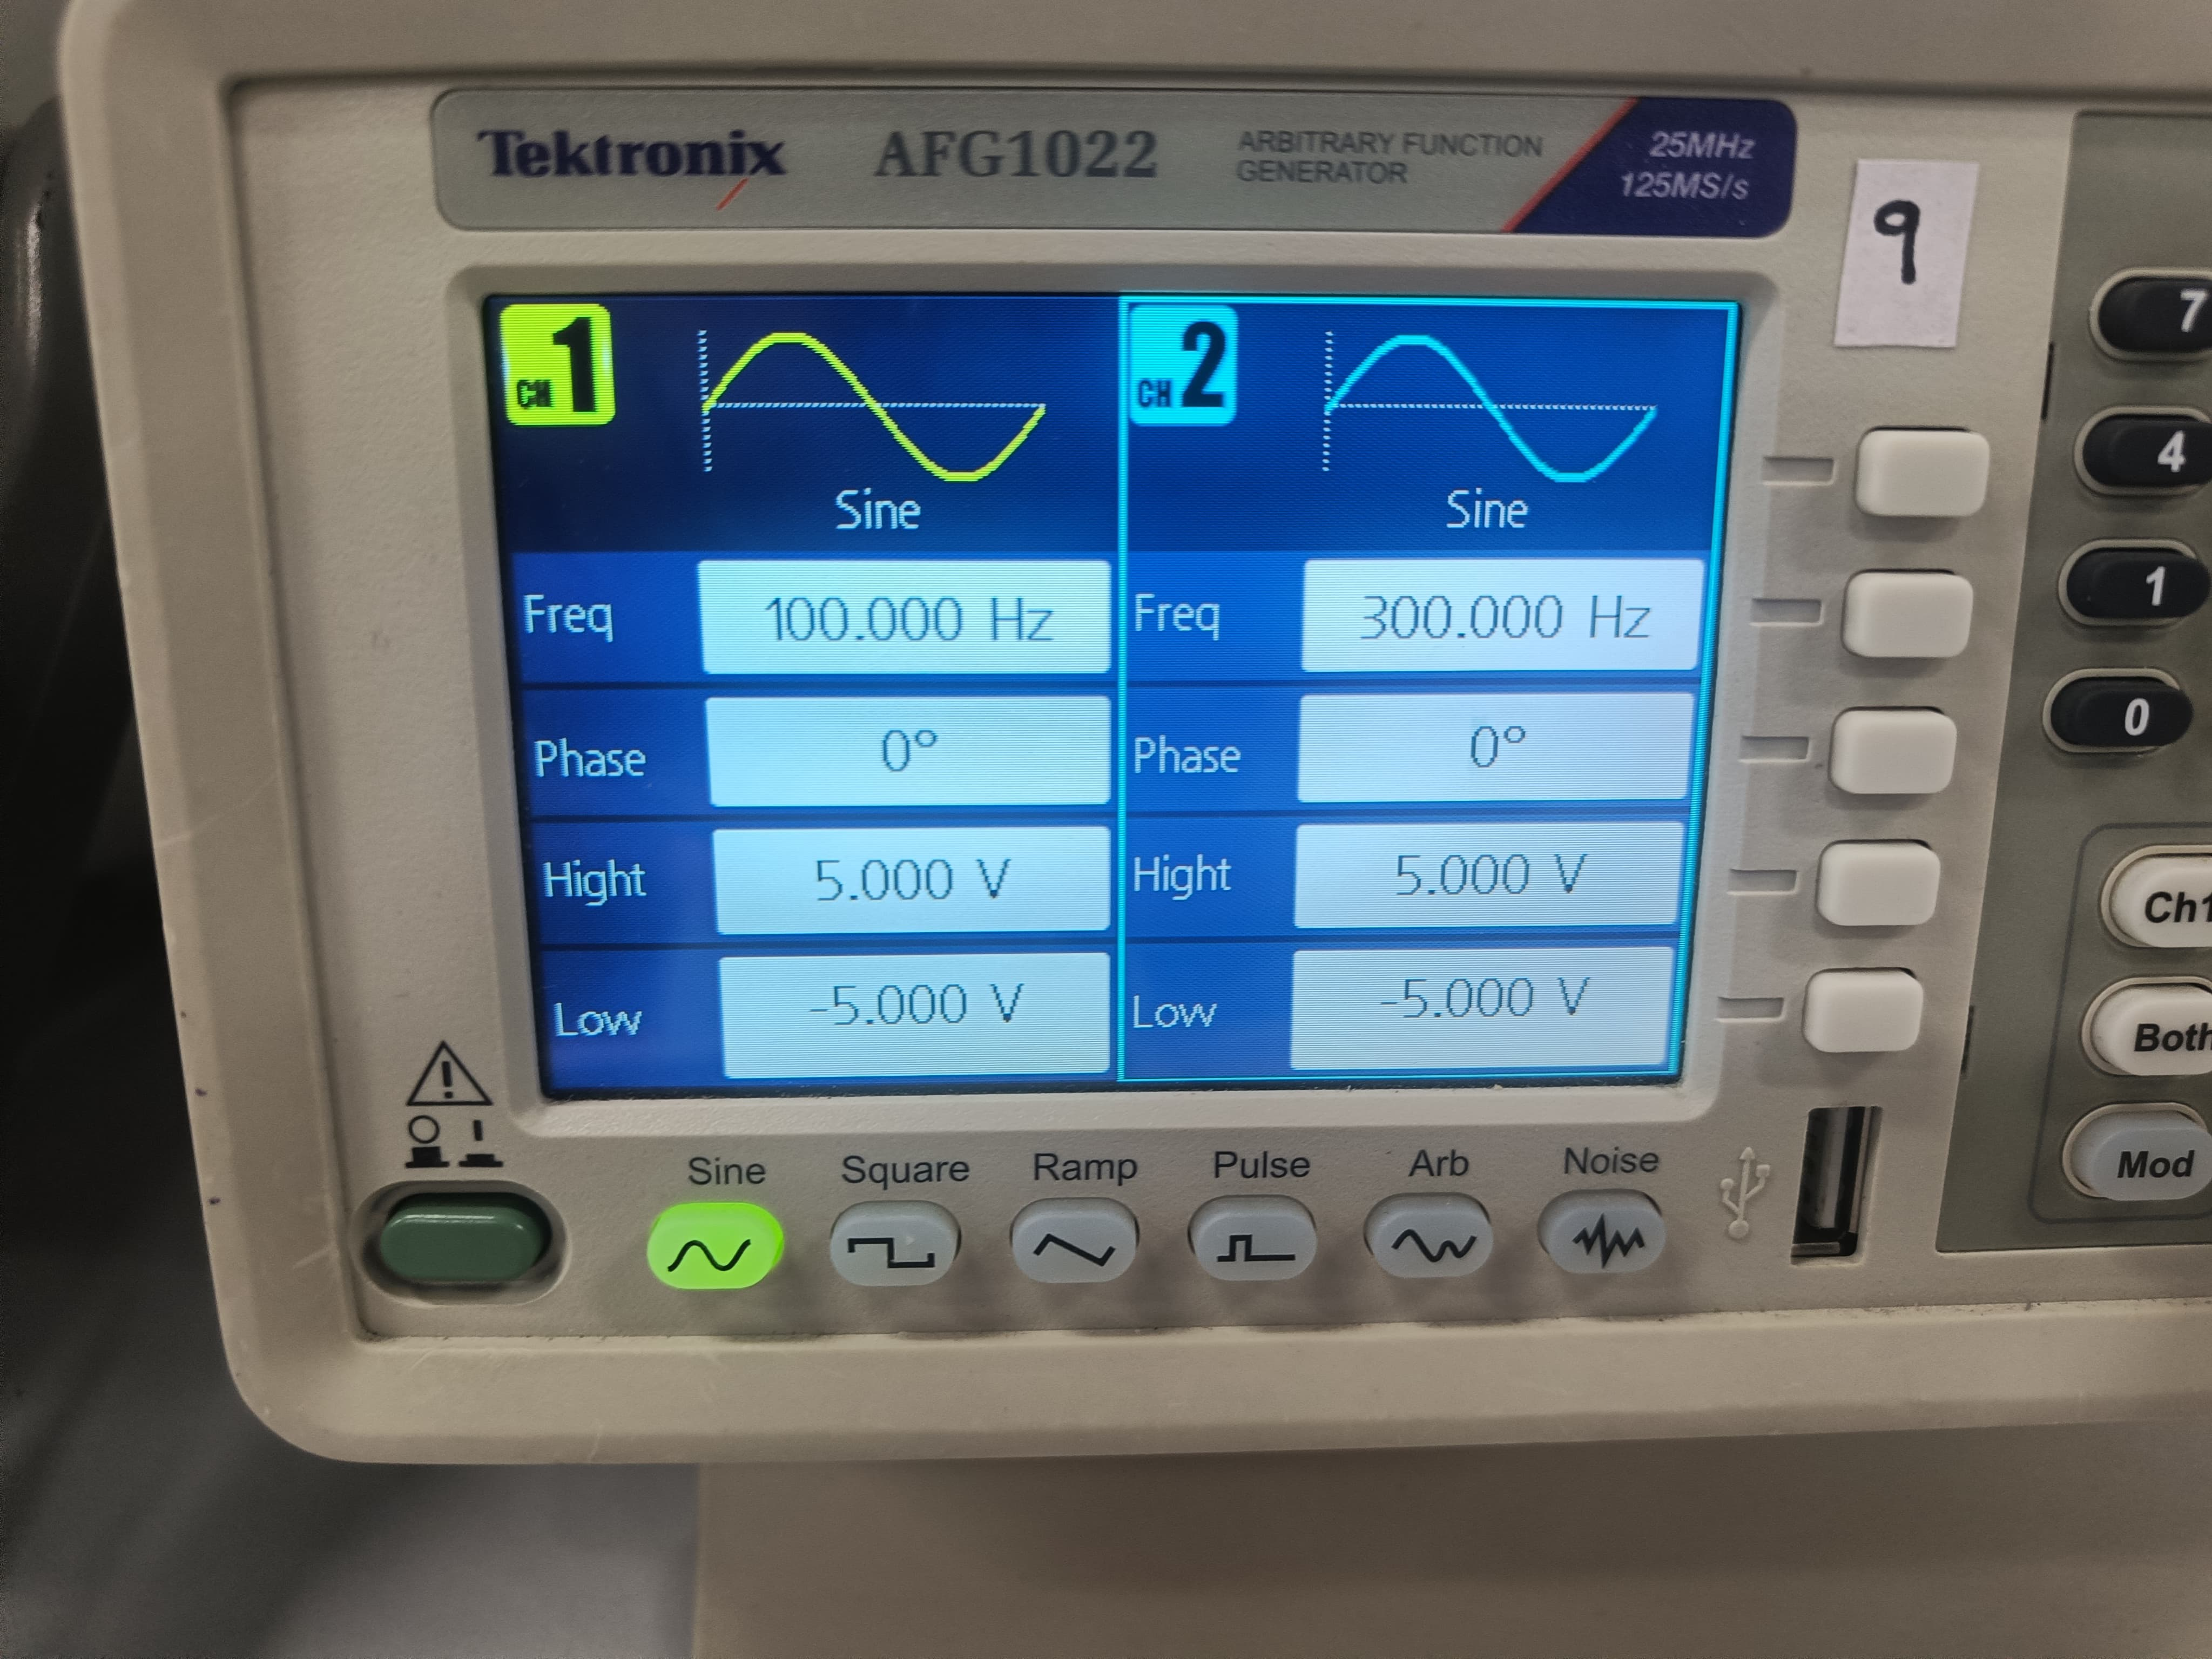
\includegraphics[width=0.7\columnwidth]{pics/WhatsApp Image 2025-01-24 at 11.02.16.jpeg}
        \caption{Input from function generator}
    \end{figure}
    \begin{figure}[H]
        \centering
        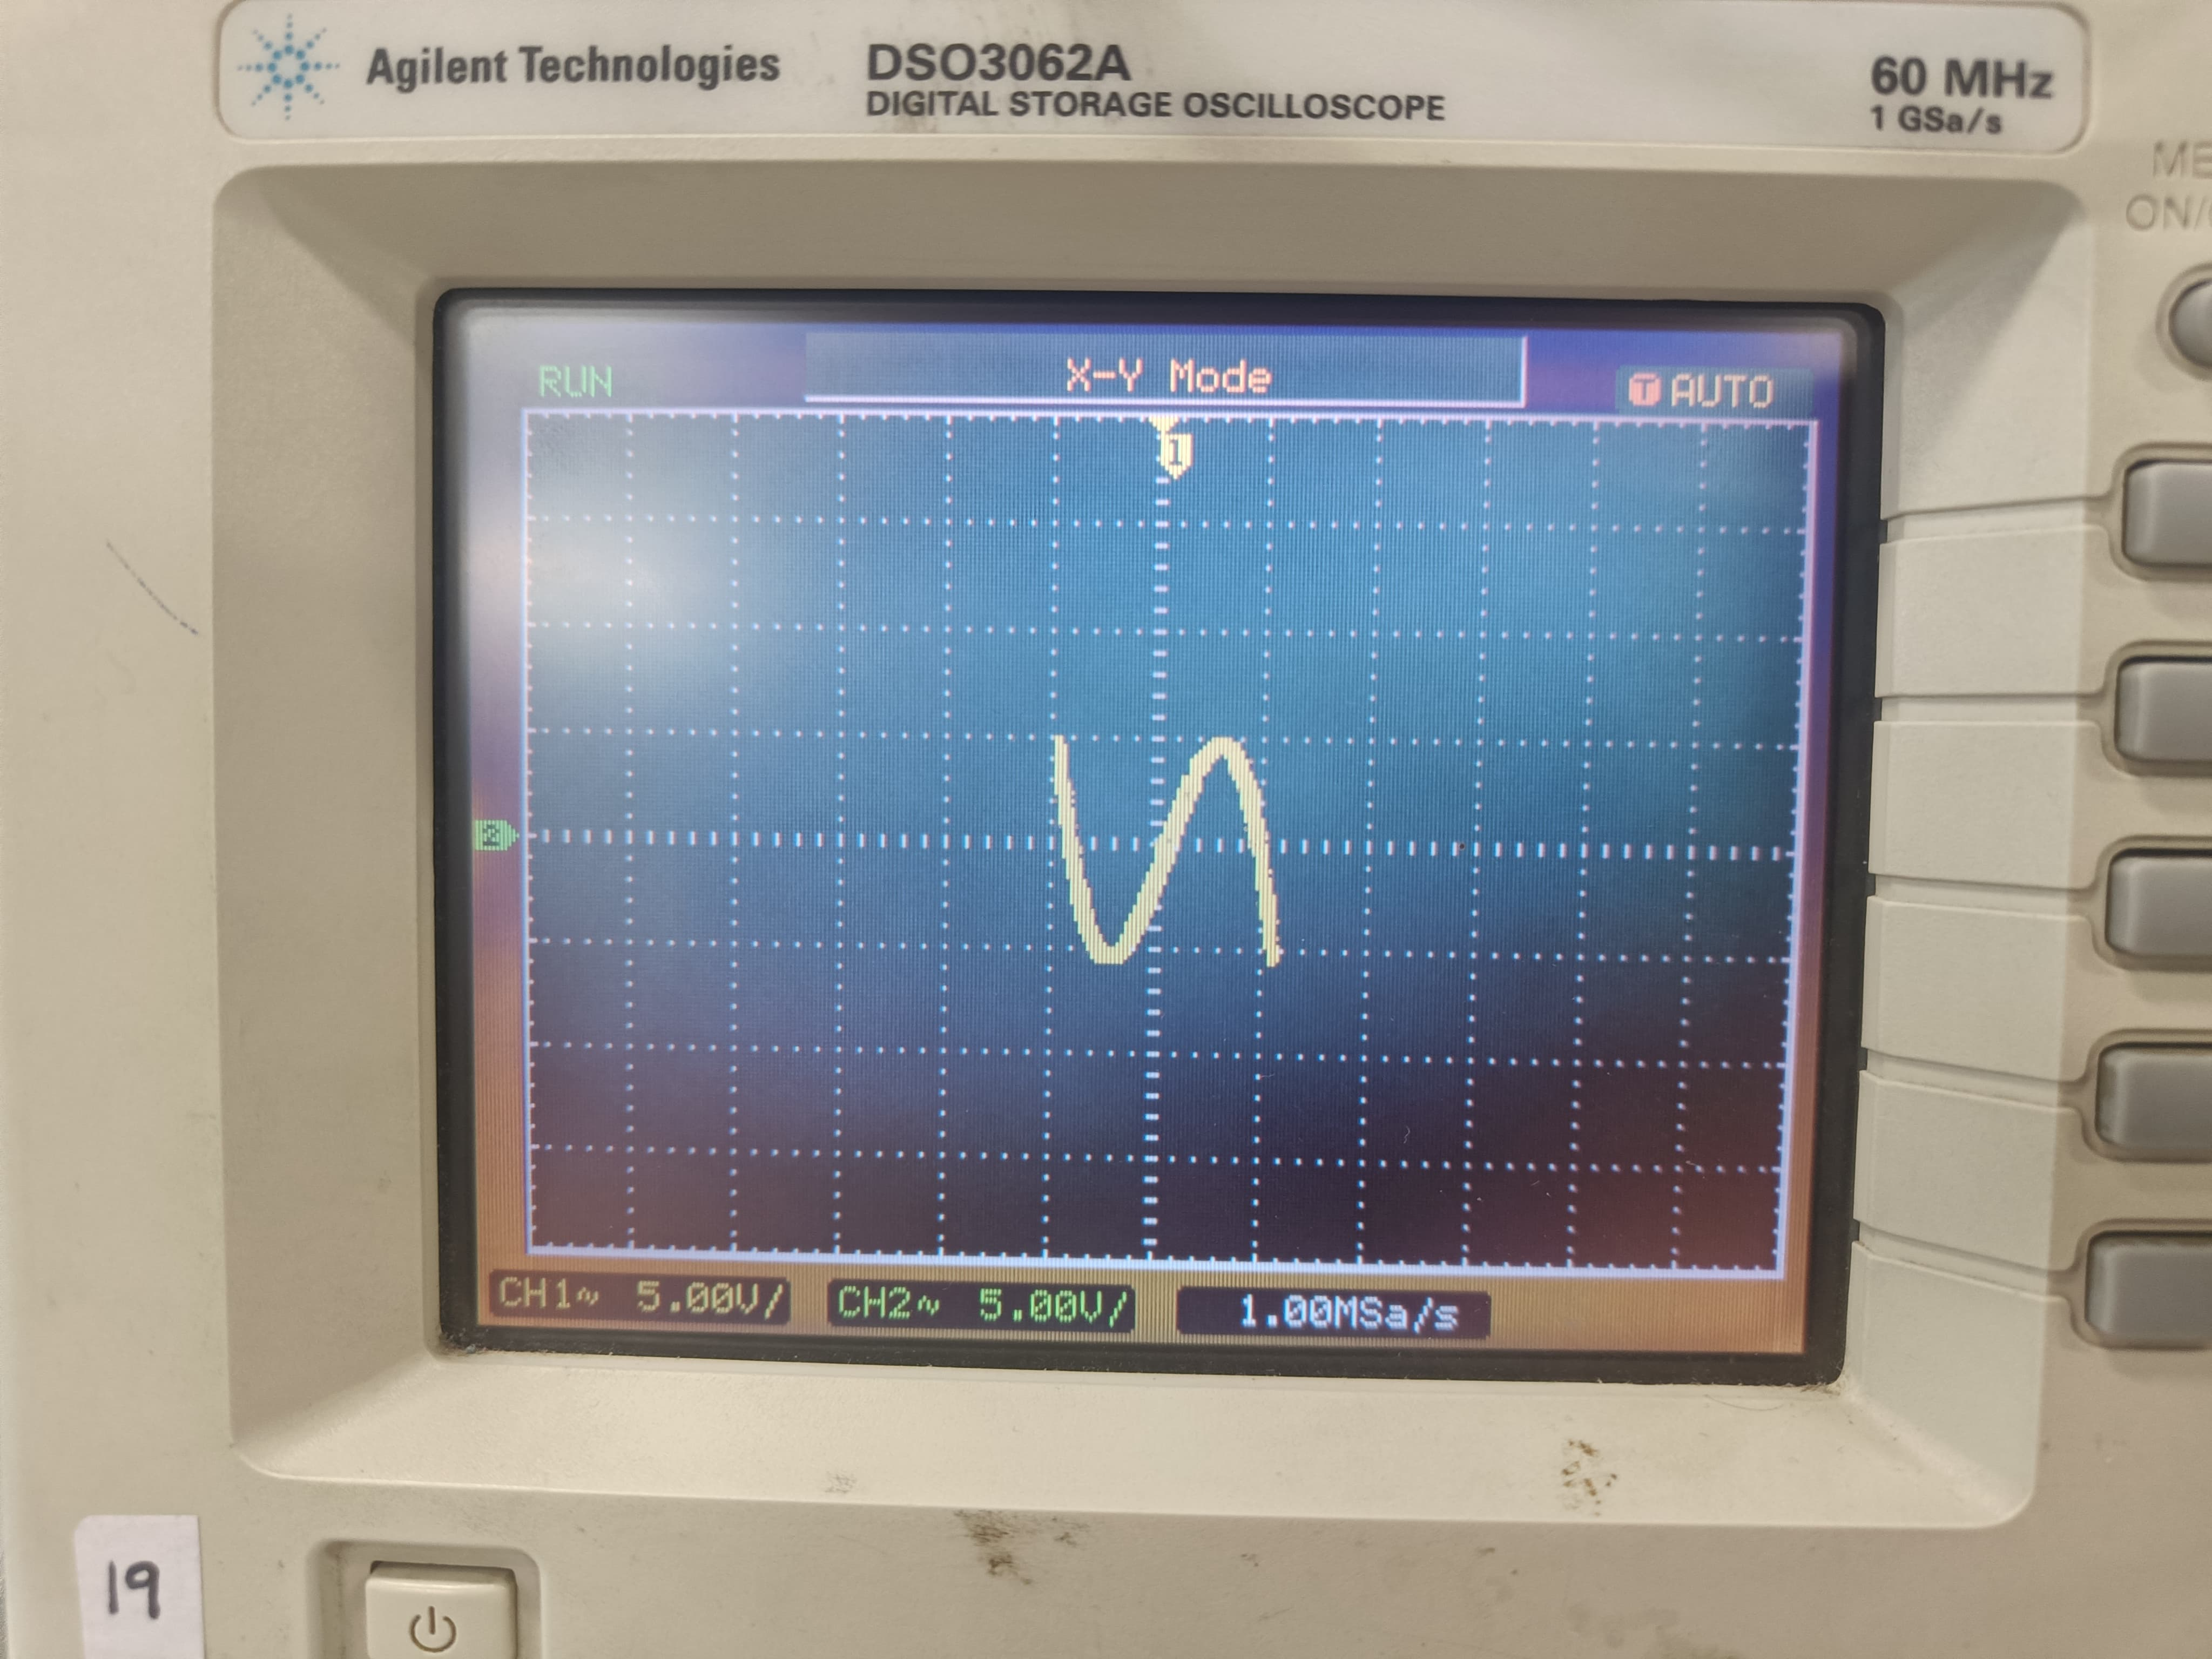
\includegraphics[width=0.7\columnwidth]{pics/WhatsApp Image 2025-01-24 at 11.02.14.jpeg}
        \caption{Output on CRO}
    \end{figure}
    \begin{figure}[H]
        \centering
        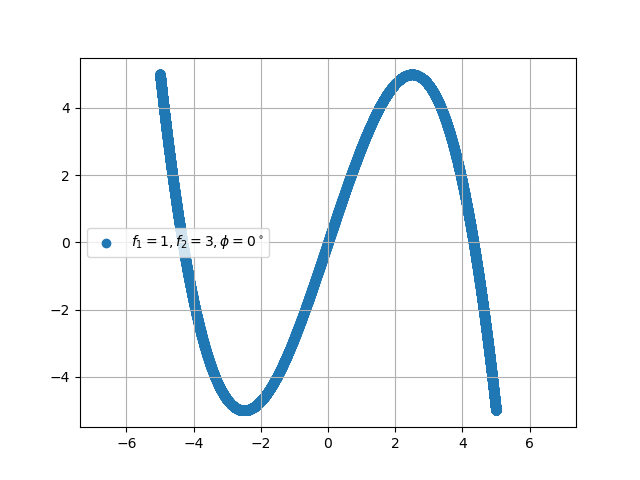
\includegraphics[width=0.7\columnwidth]{figs/fig5.png}
        \caption{Theoretical Plot}
    \end{figure}
%6
    \item \begin{align}
        x = 5\sin\brak{\frac{2\pi}{3}t+\frac{\pi}{2}},\,y = 5\sin\brak{\frac{2\pi}{2}t}
    \end{align}
    \begin{figure}[H]
        \centering
        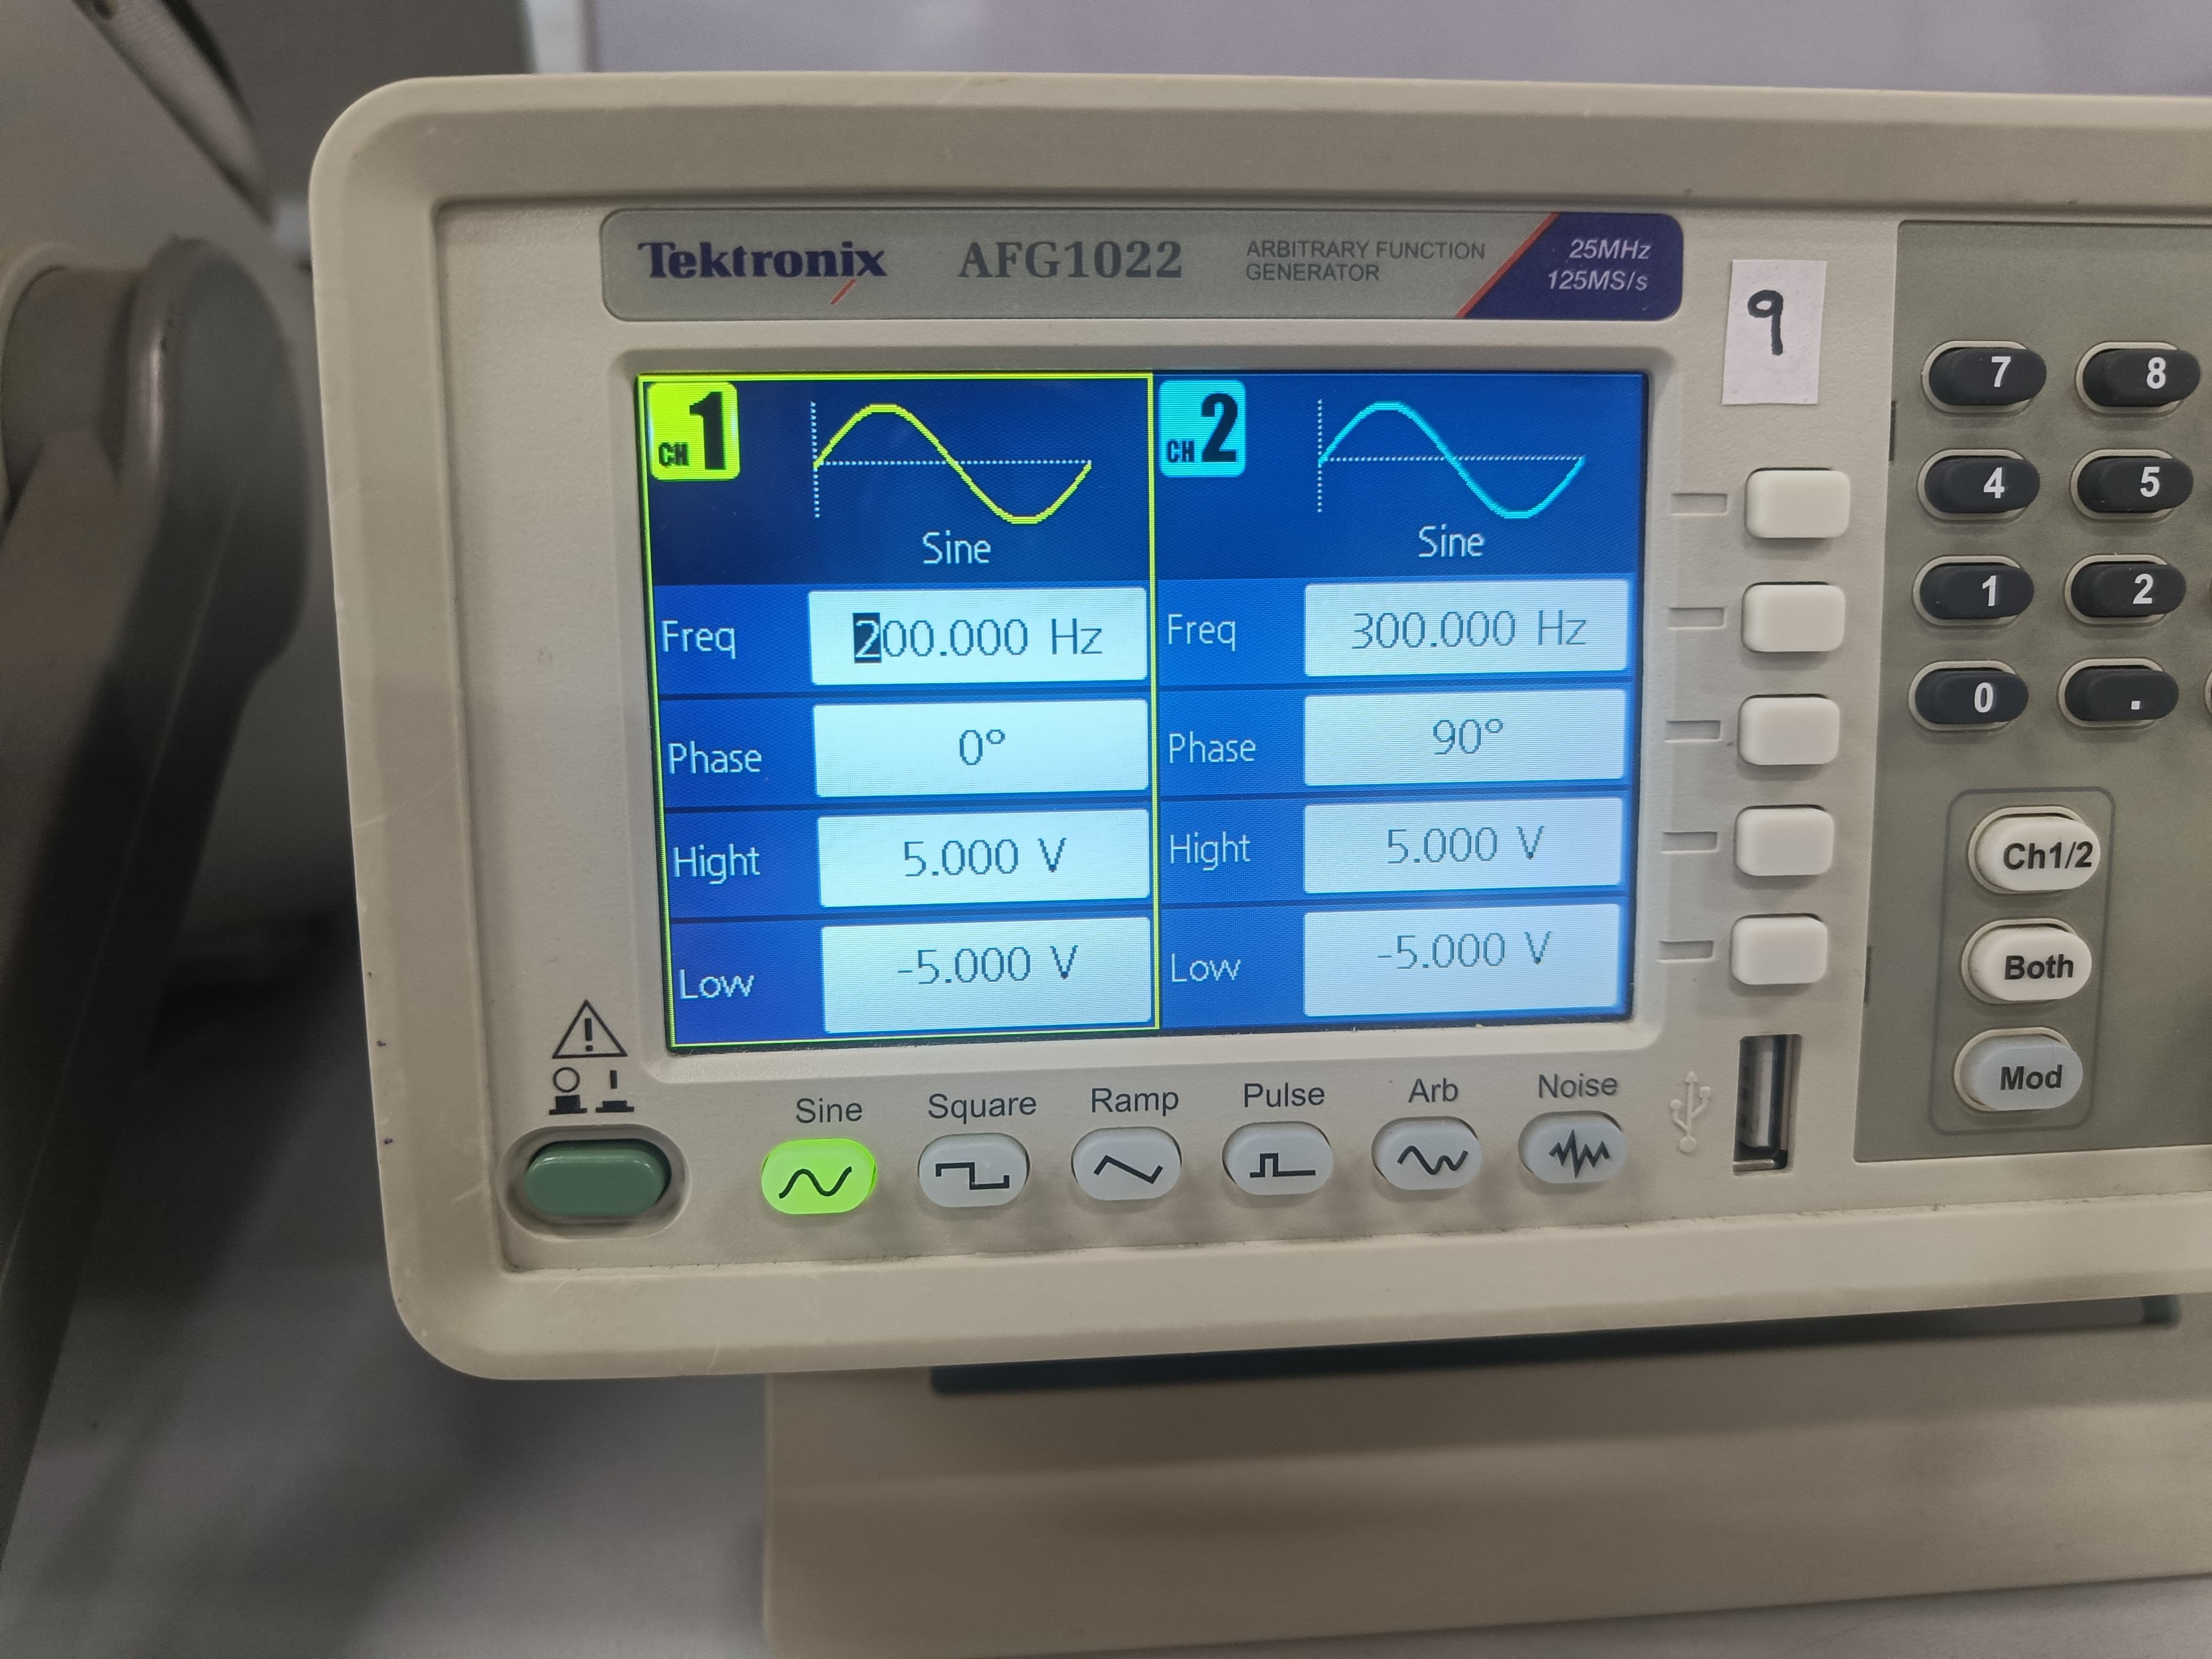
\includegraphics[width=0.7\columnwidth]{pics/WhatsApp Image 2025-01-24 at 11.02.13(1).jpeg}
        \caption{Input from function generator}
    \end{figure}
    \begin{figure}[H]
        \centering
        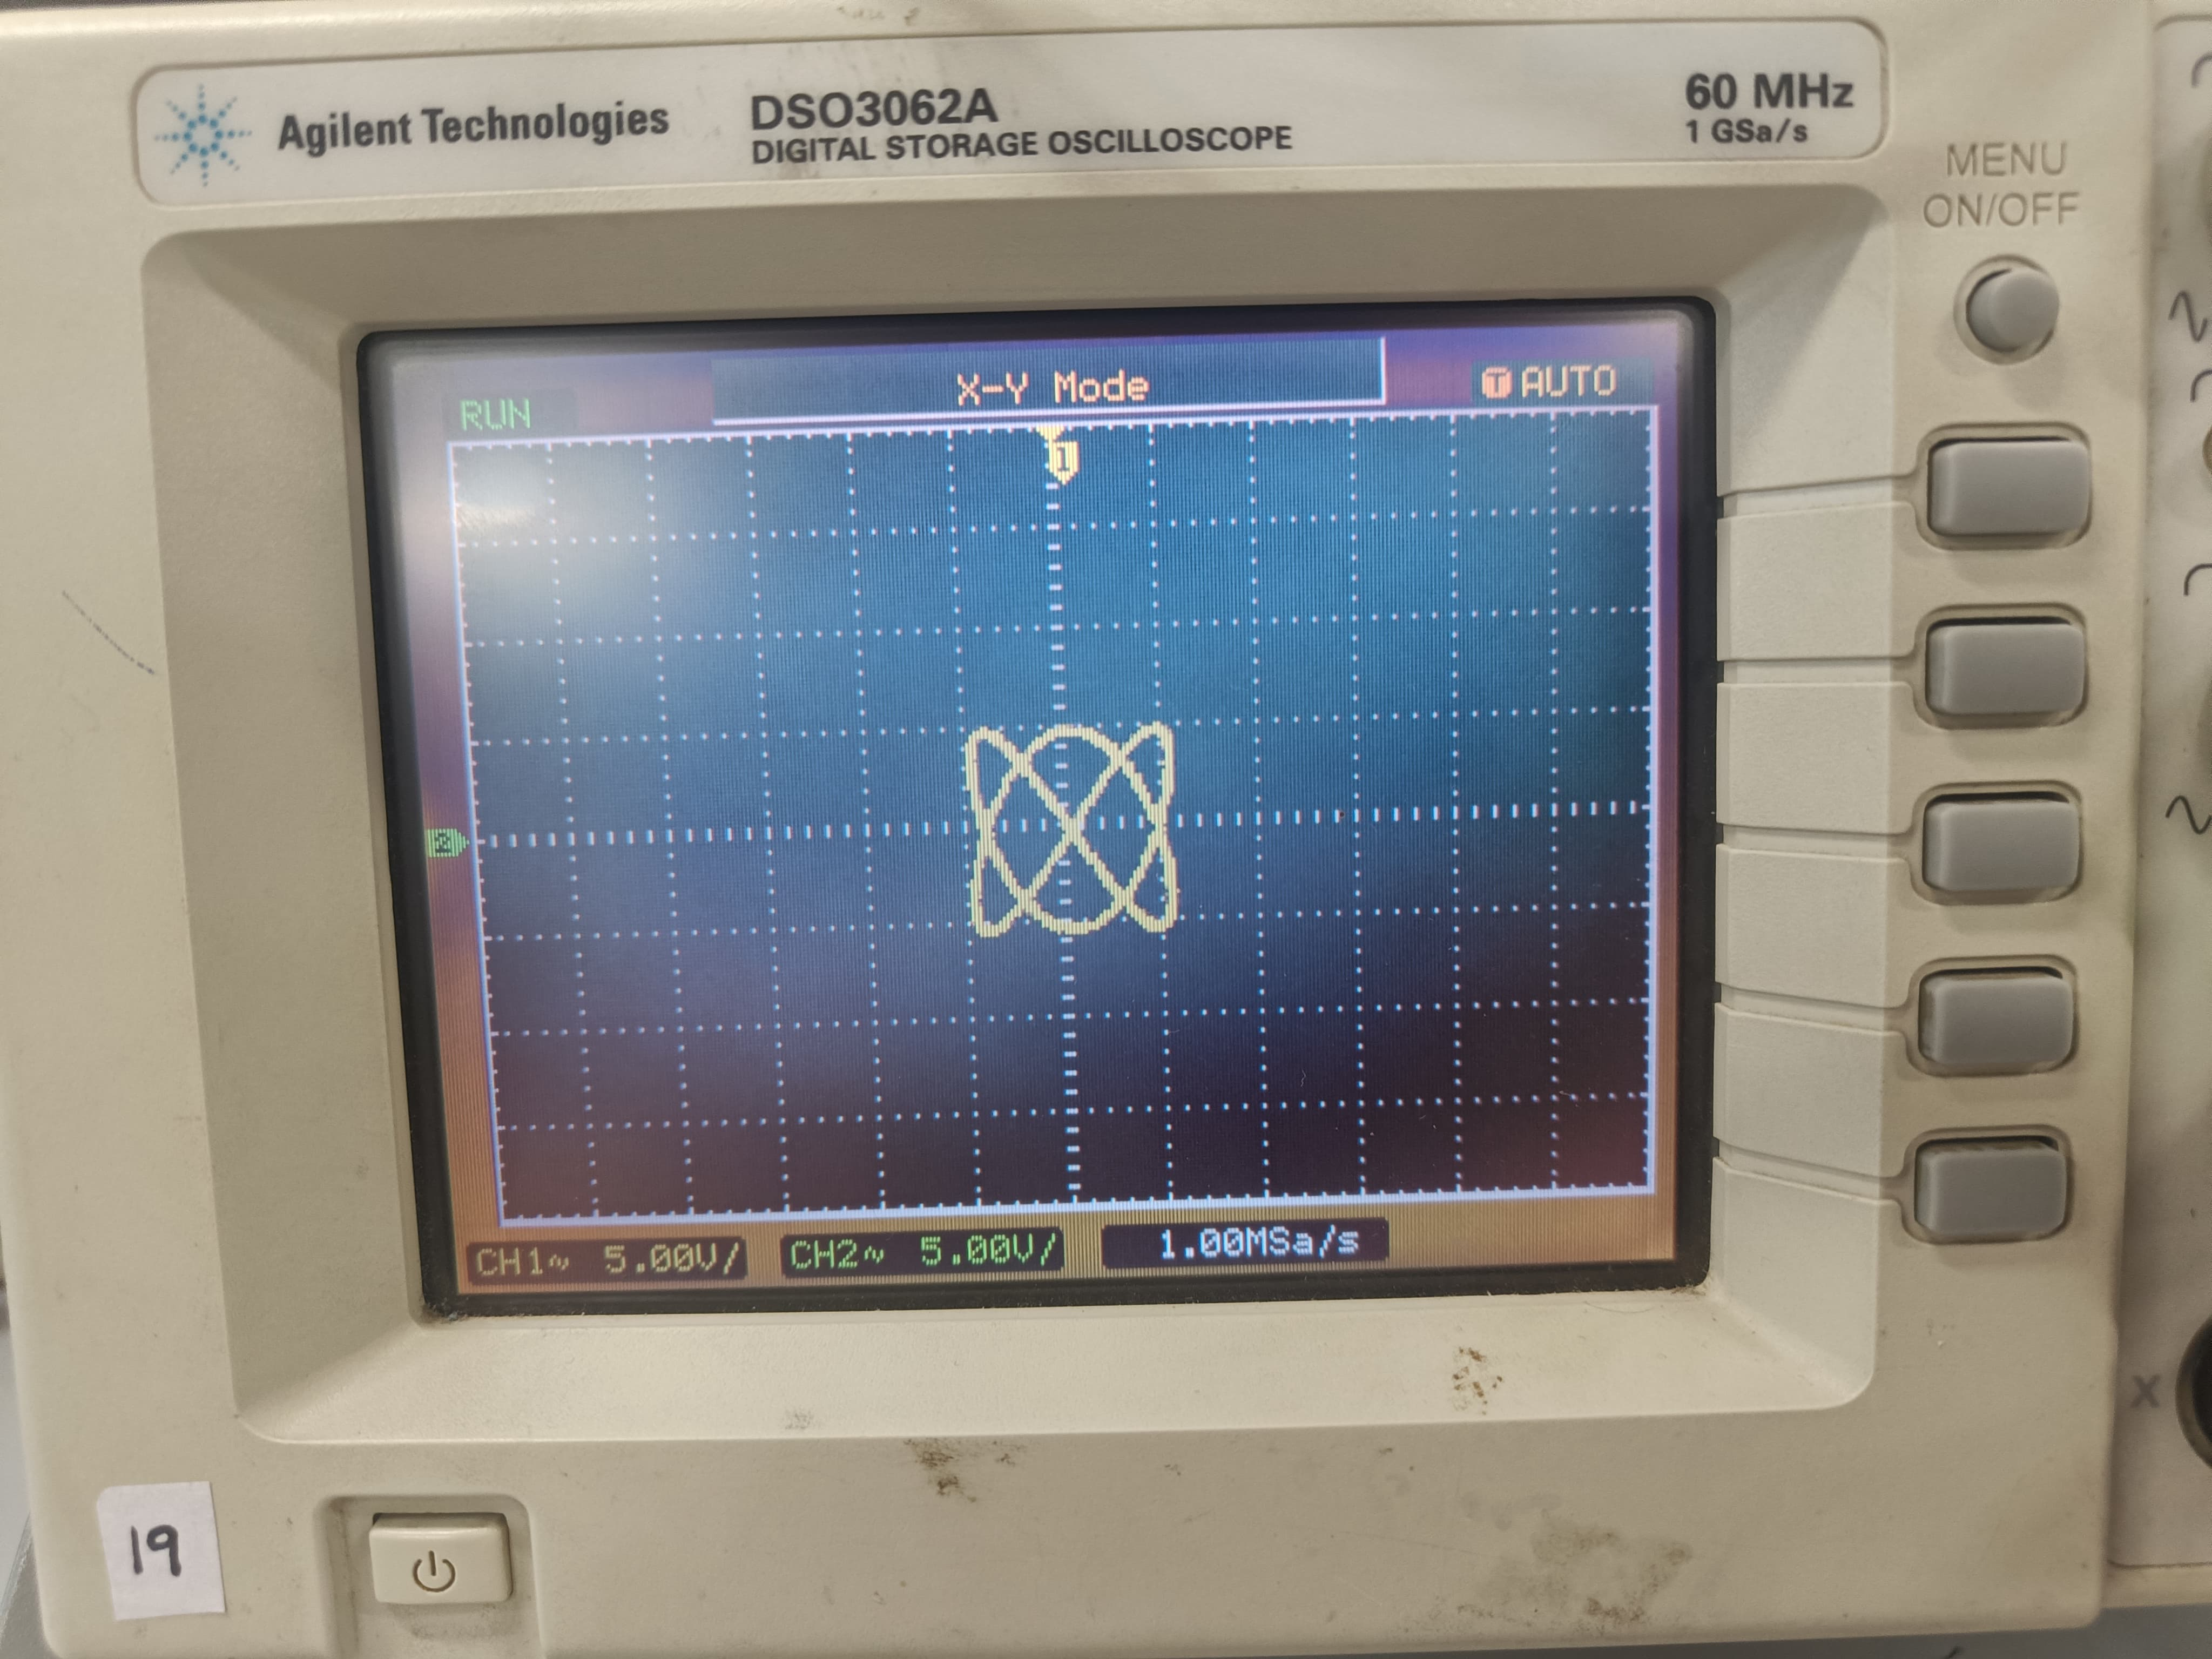
\includegraphics[width=0.7\columnwidth]{pics/WhatsApp Image 2025-01-24 at 11.02.13.jpeg}
        \caption{Output on CRO}
    \end{figure}
    \begin{figure}[H]
        \centering
        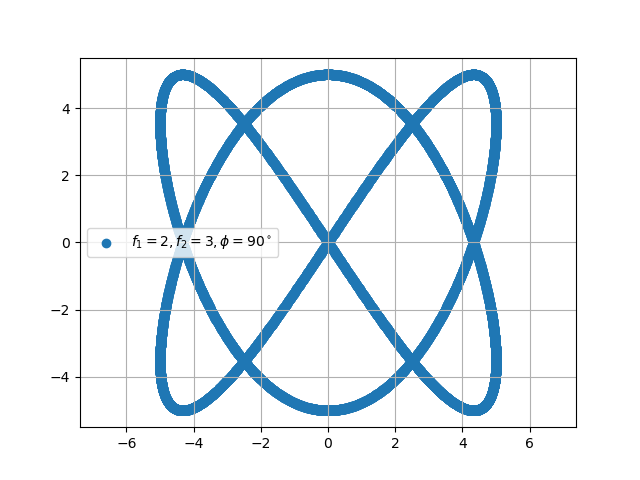
\includegraphics[width=0.7\columnwidth]{figs/fig6.png}
        \caption{Theoretical Plot}
    \end{figure}
%7
    \item \begin{align}
        x = 5\sin\brak{\frac{2\pi}{2}t+\frac{\pi}{2}},\,y = 5\sin\brak{{2\pi}t}
    \end{align}
    \begin{figure}[H]
        \centering
        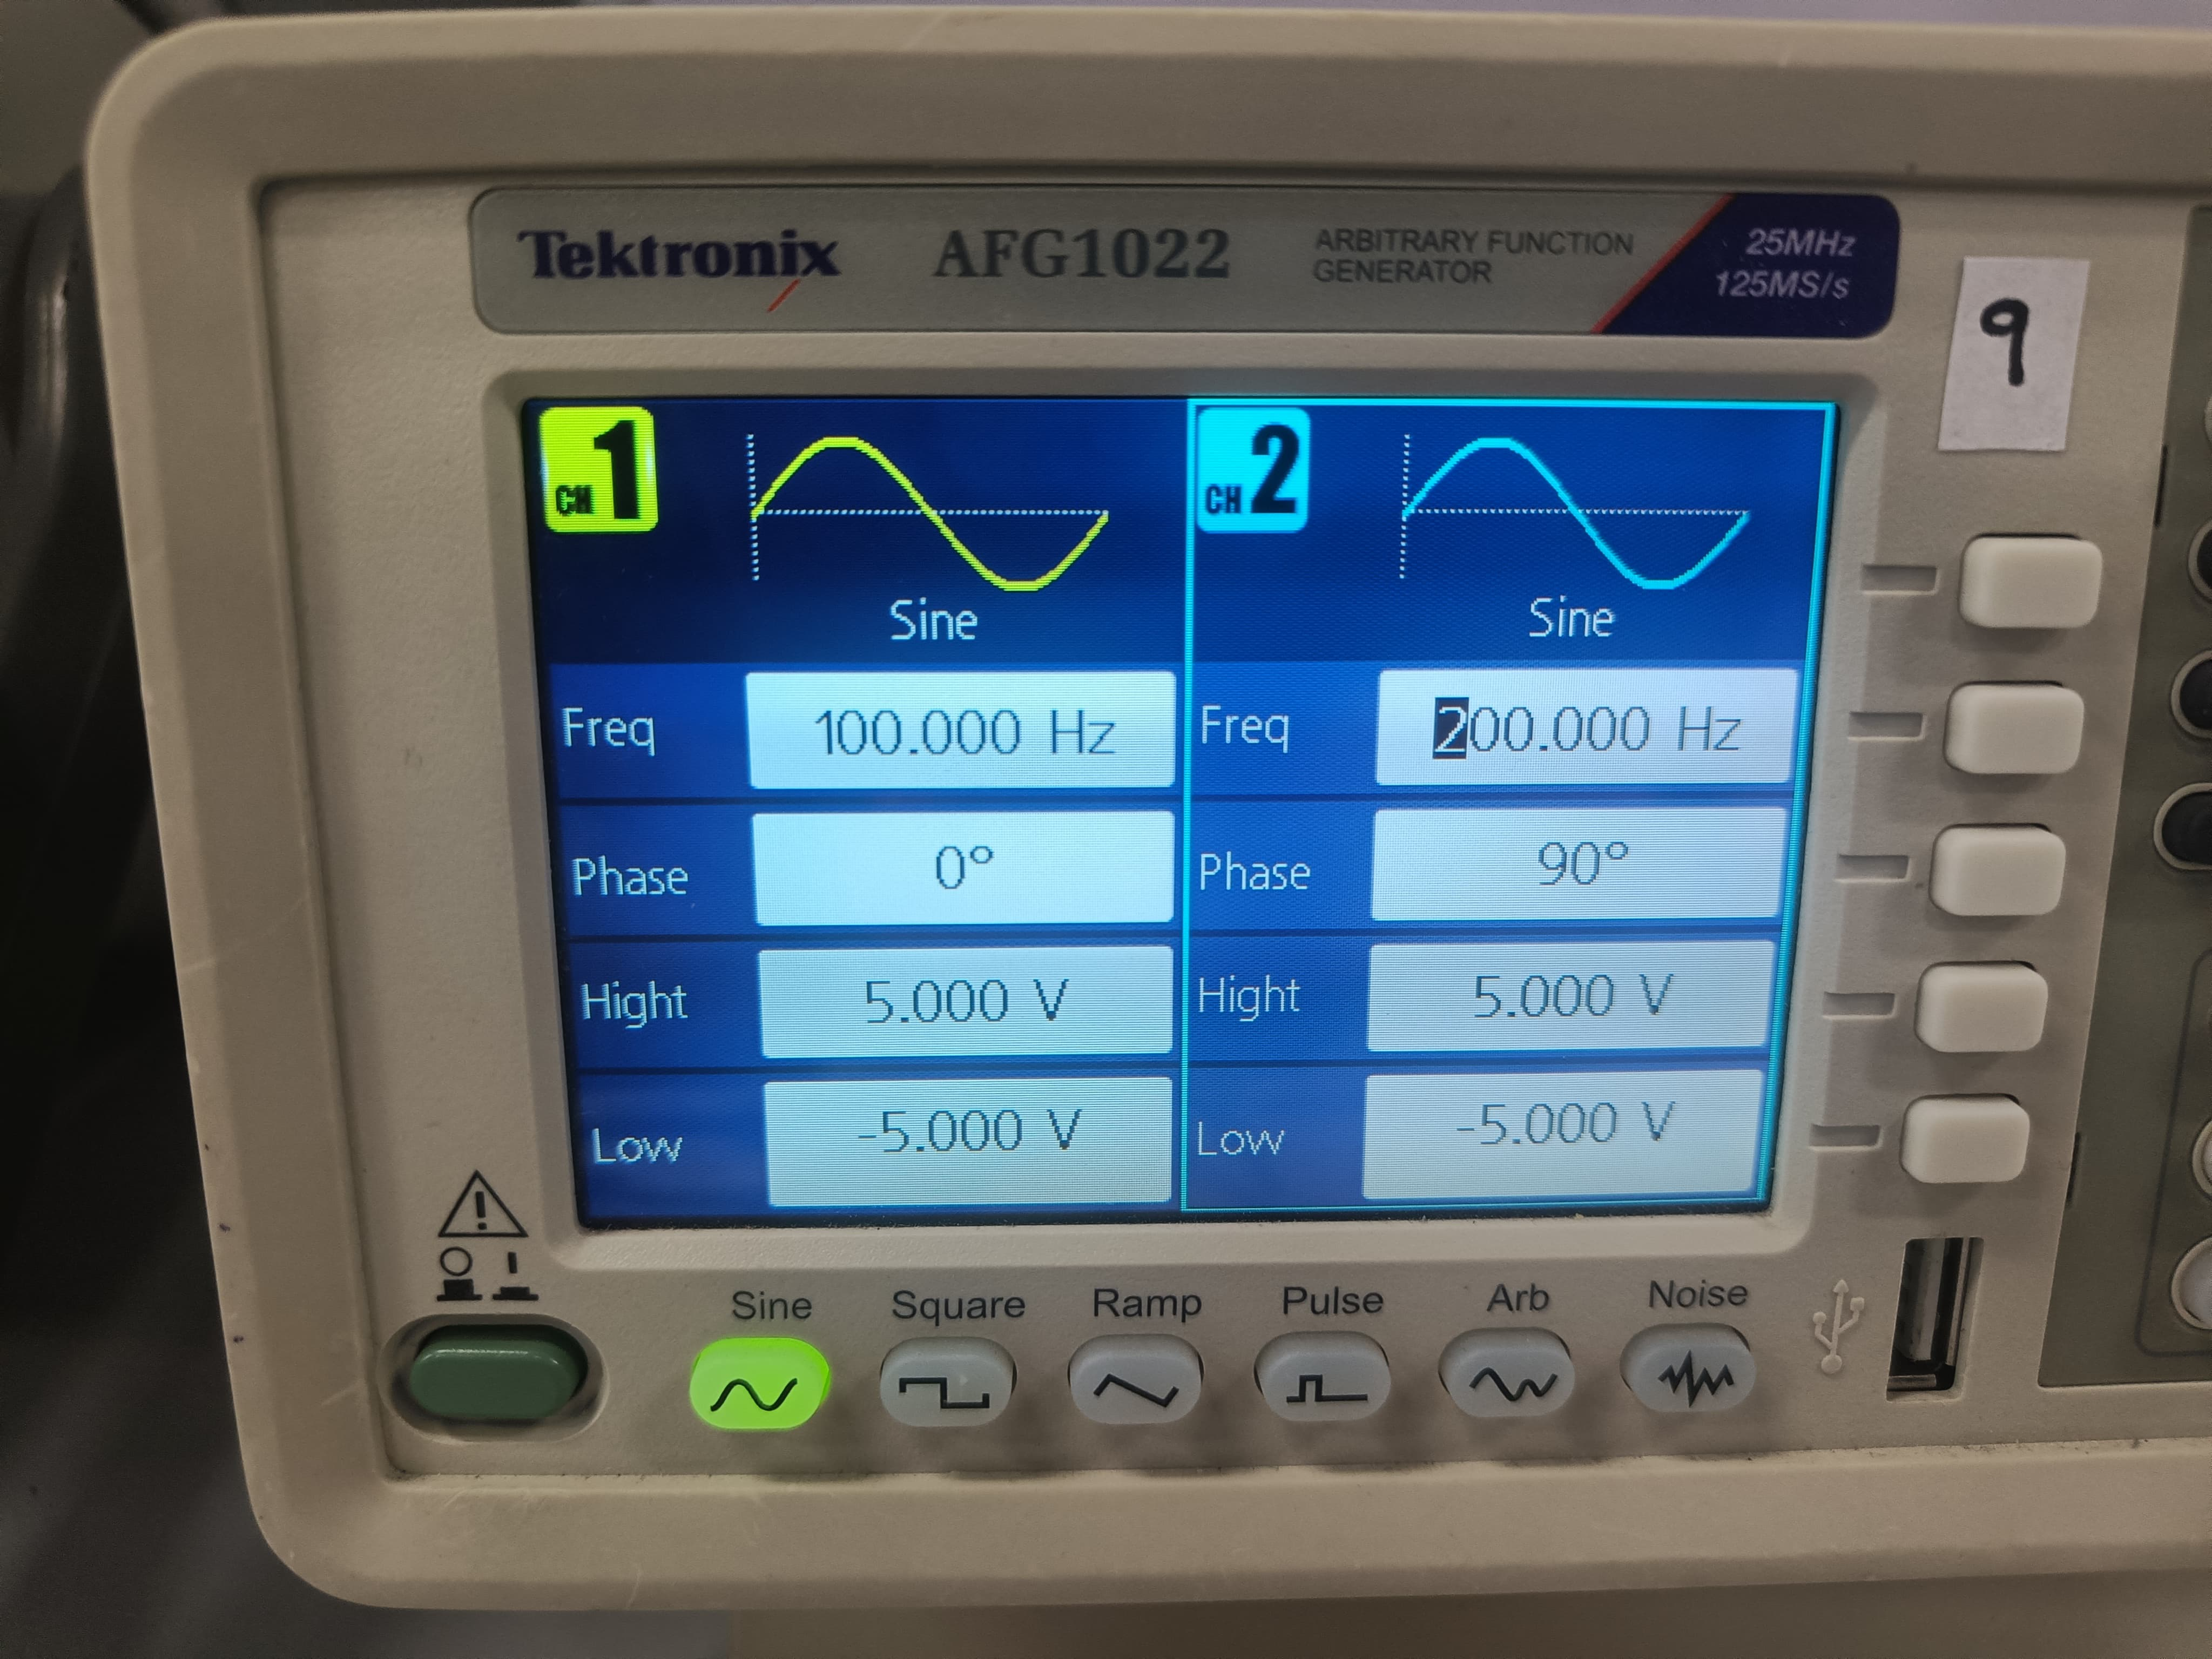
\includegraphics[width=0.7\columnwidth]{pics/WhatsApp Image 2025-01-24 at 11.02.12(1).jpeg}
        \caption{Input from function generator}
    \end{figure}
    \begin{figure}[H]
        \centering
        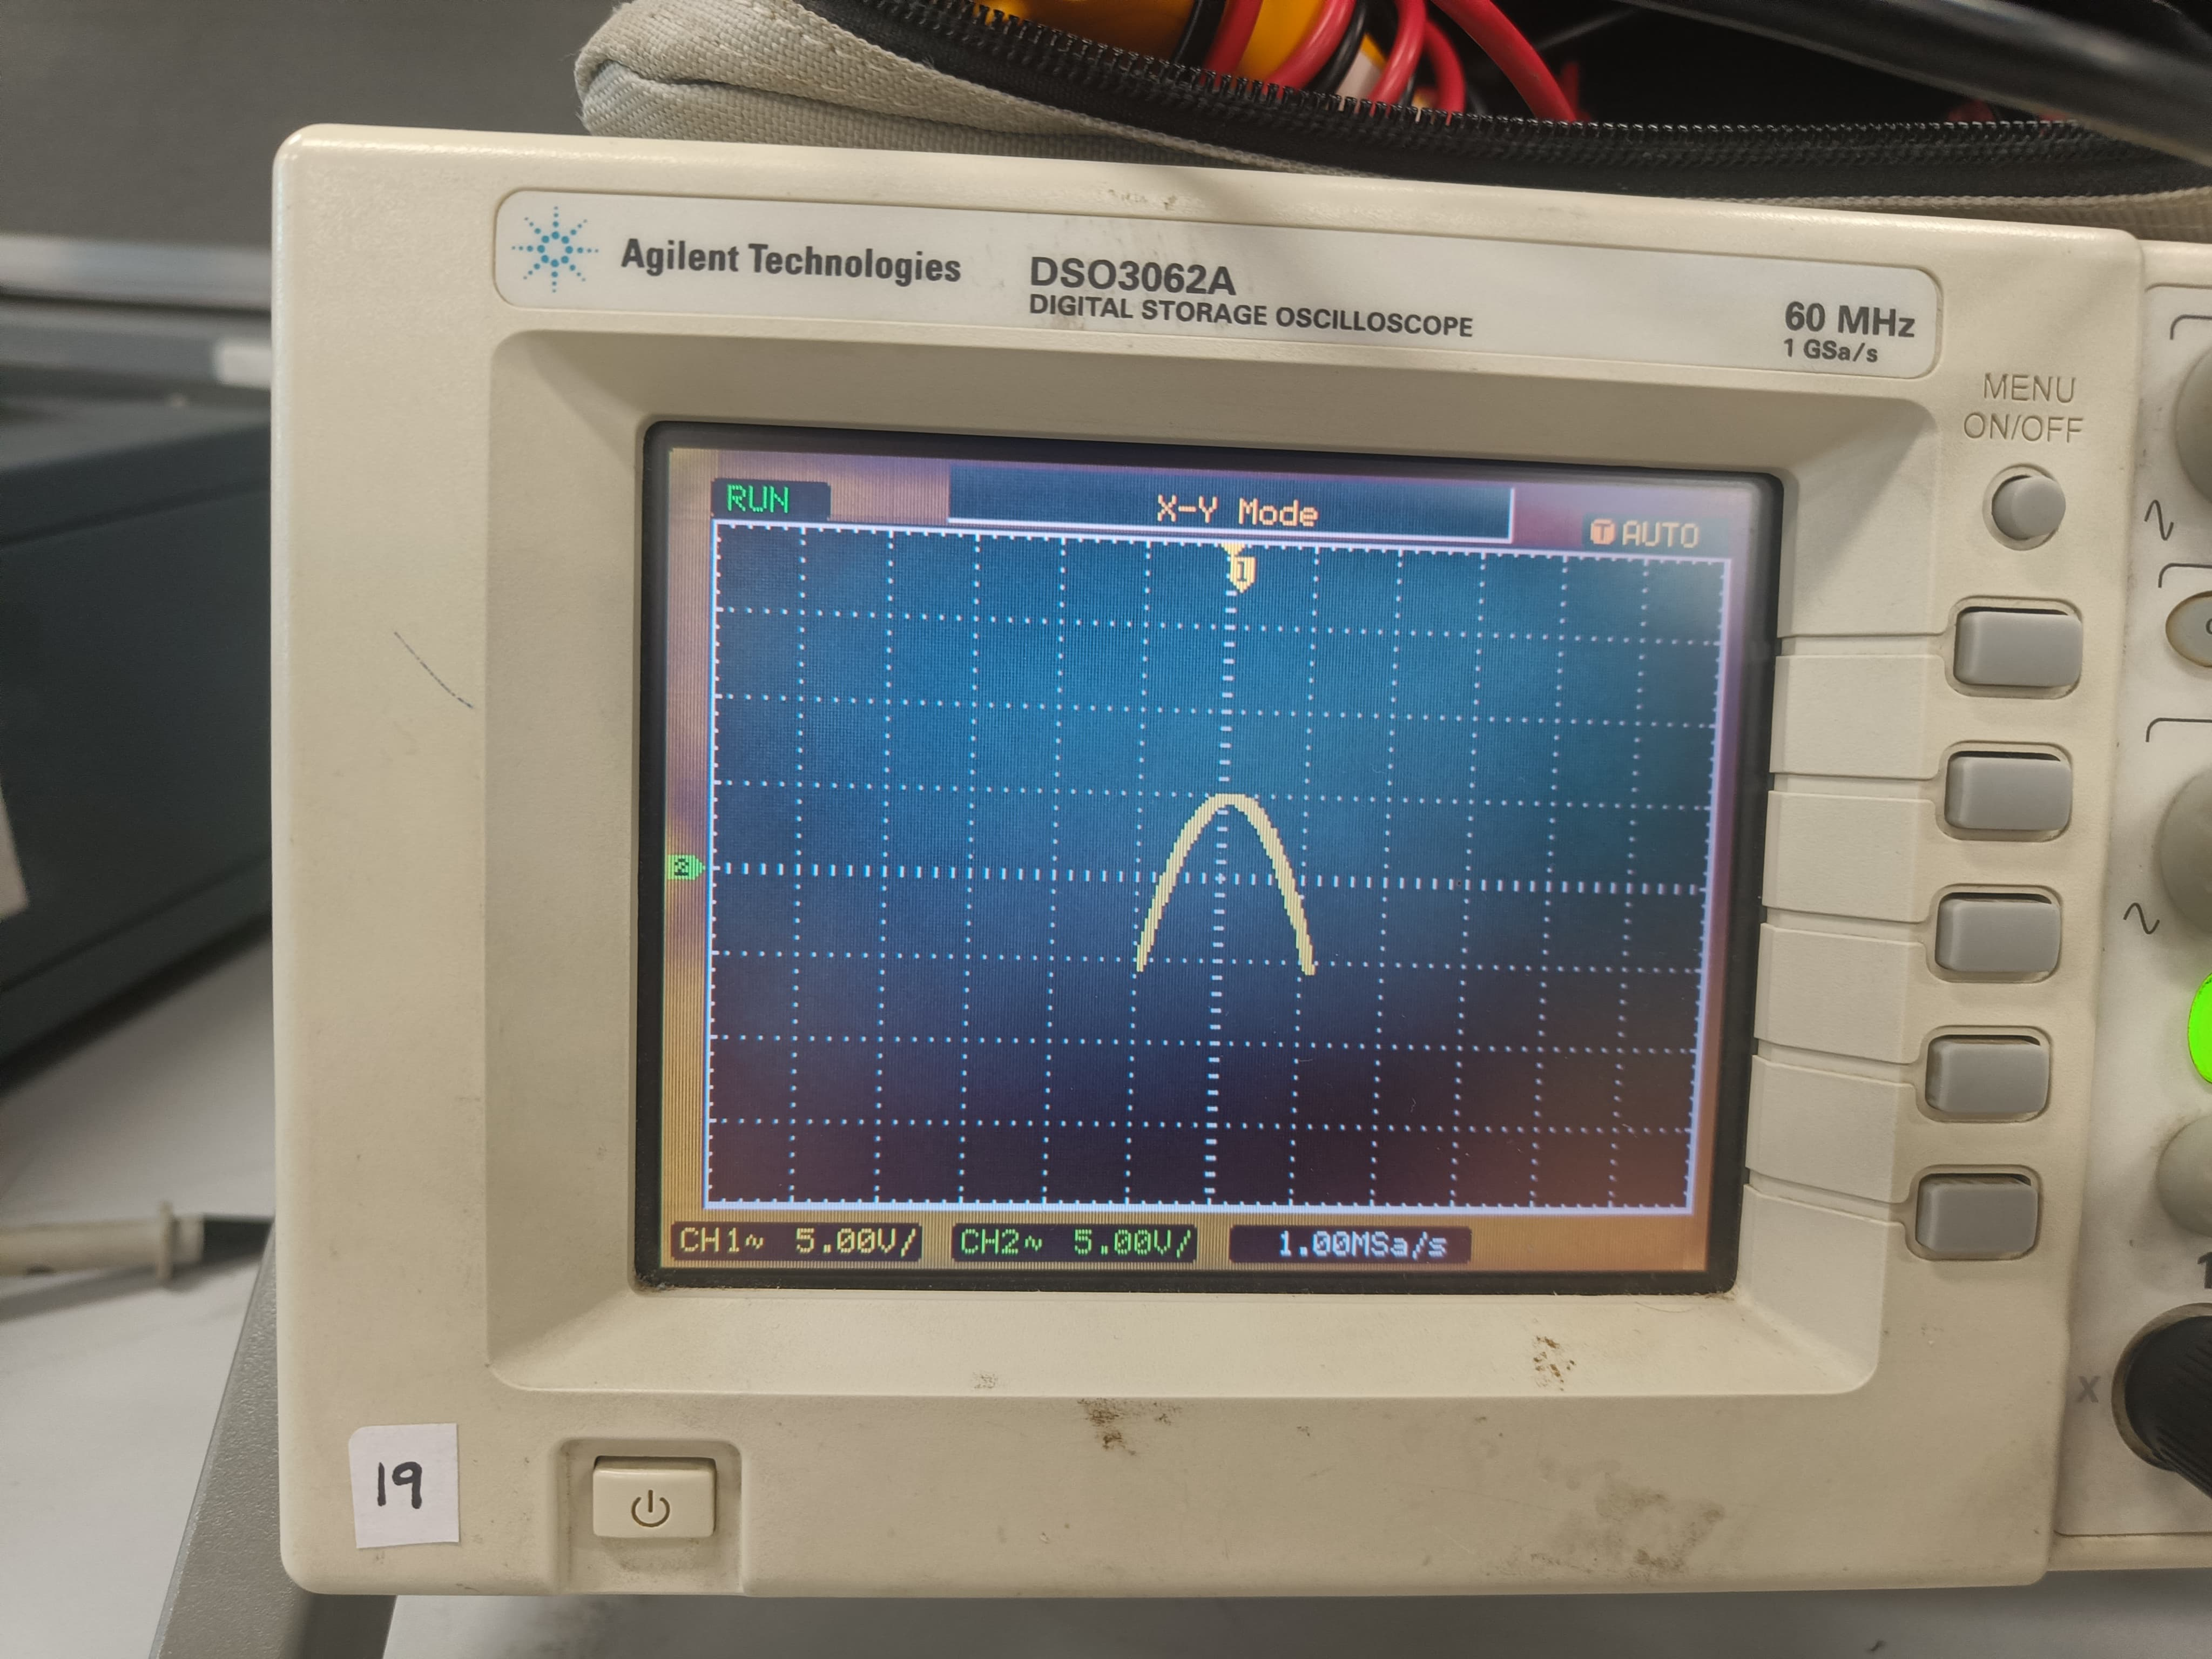
\includegraphics[width=0.7\columnwidth]{pics/WhatsApp Image 2025-01-24 at 11.02.12.jpeg}
        \caption{Output on CRO}
    \end{figure}
    \begin{figure}[H]
        \centering
        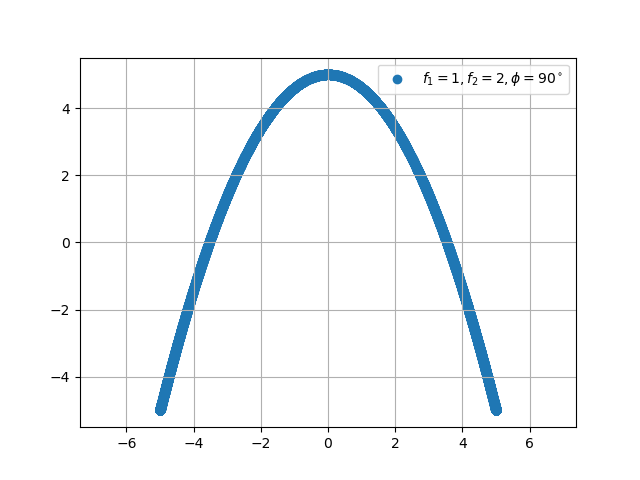
\includegraphics[width=0.7\columnwidth]{figs/fig7.png}
        \caption{Theoretical Plot}
    \end{figure}
%8
    \item \begin{align}
        x = 5\sin\brak{\frac{2\pi}{6}t},\,y = 5\sin\brak{\frac{2\pi}{5}t}
    \end{align}
    \begin{figure}[H]
        \centering
        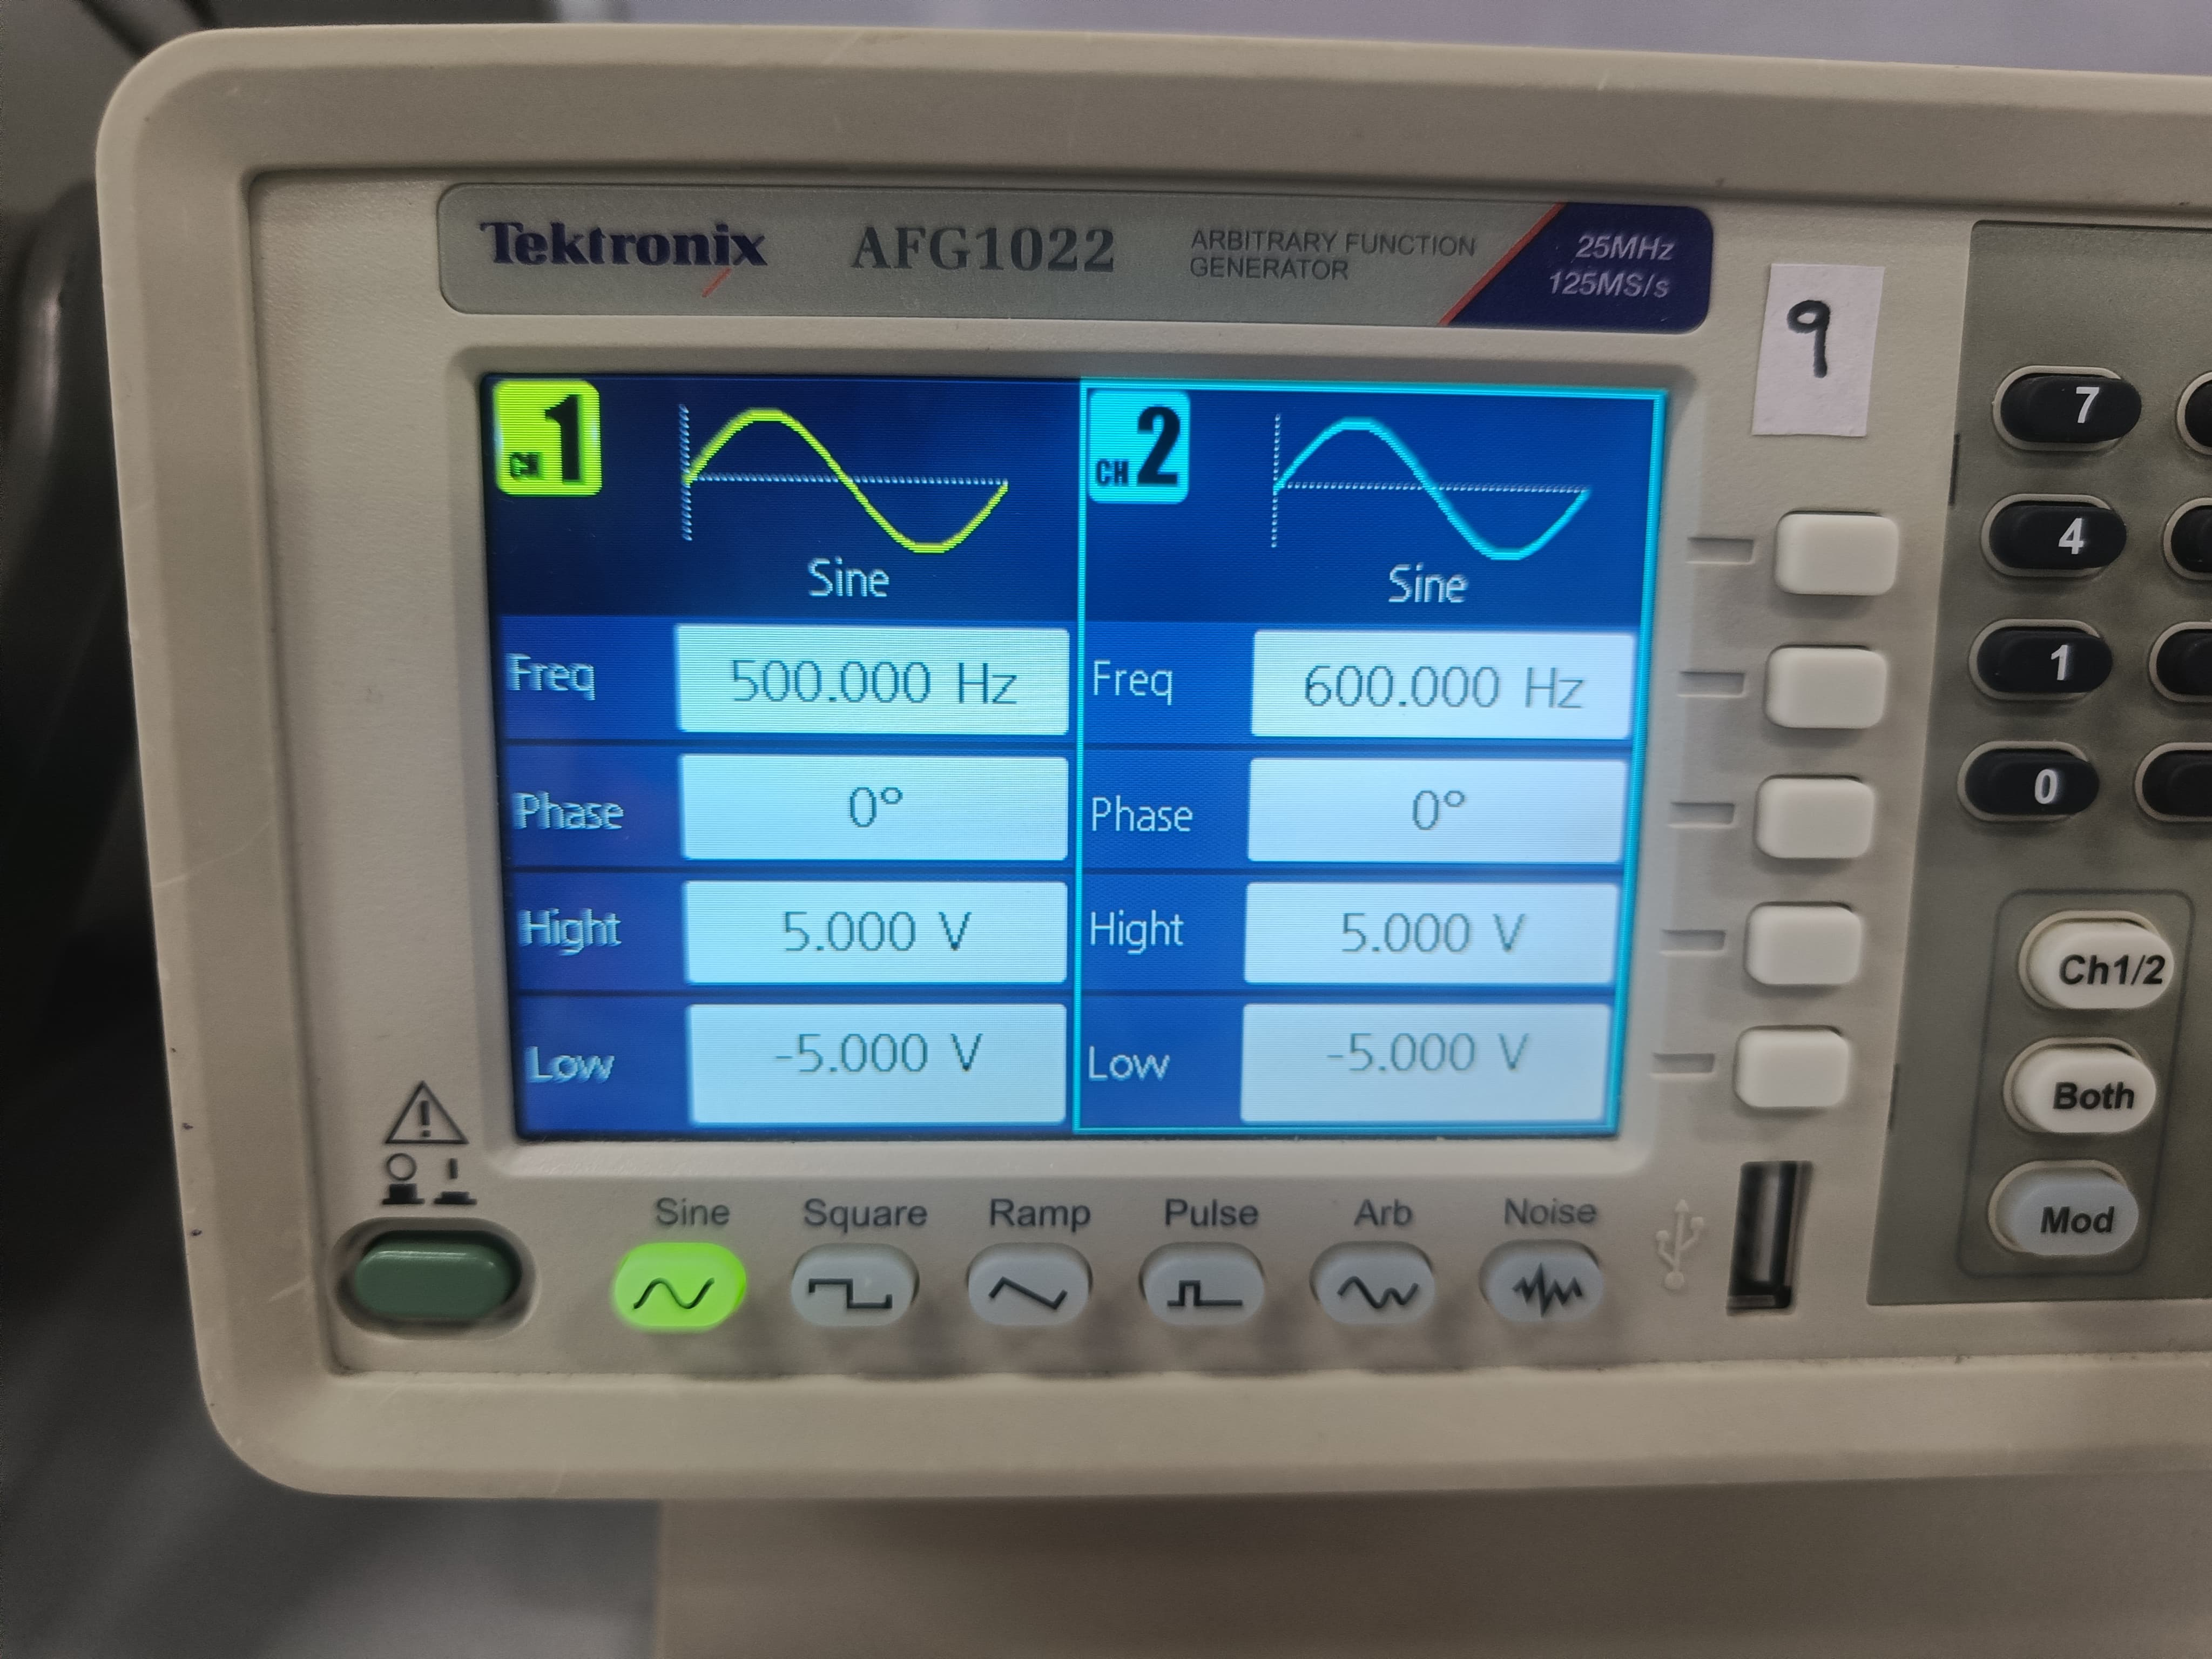
\includegraphics[width=0.7\columnwidth]{pics/WhatsApp Image 2025-01-24 at 11.02.11(1).jpeg}
        \caption{Input from function generator}
    \end{figure}
    \begin{figure}[H]
        \centering
        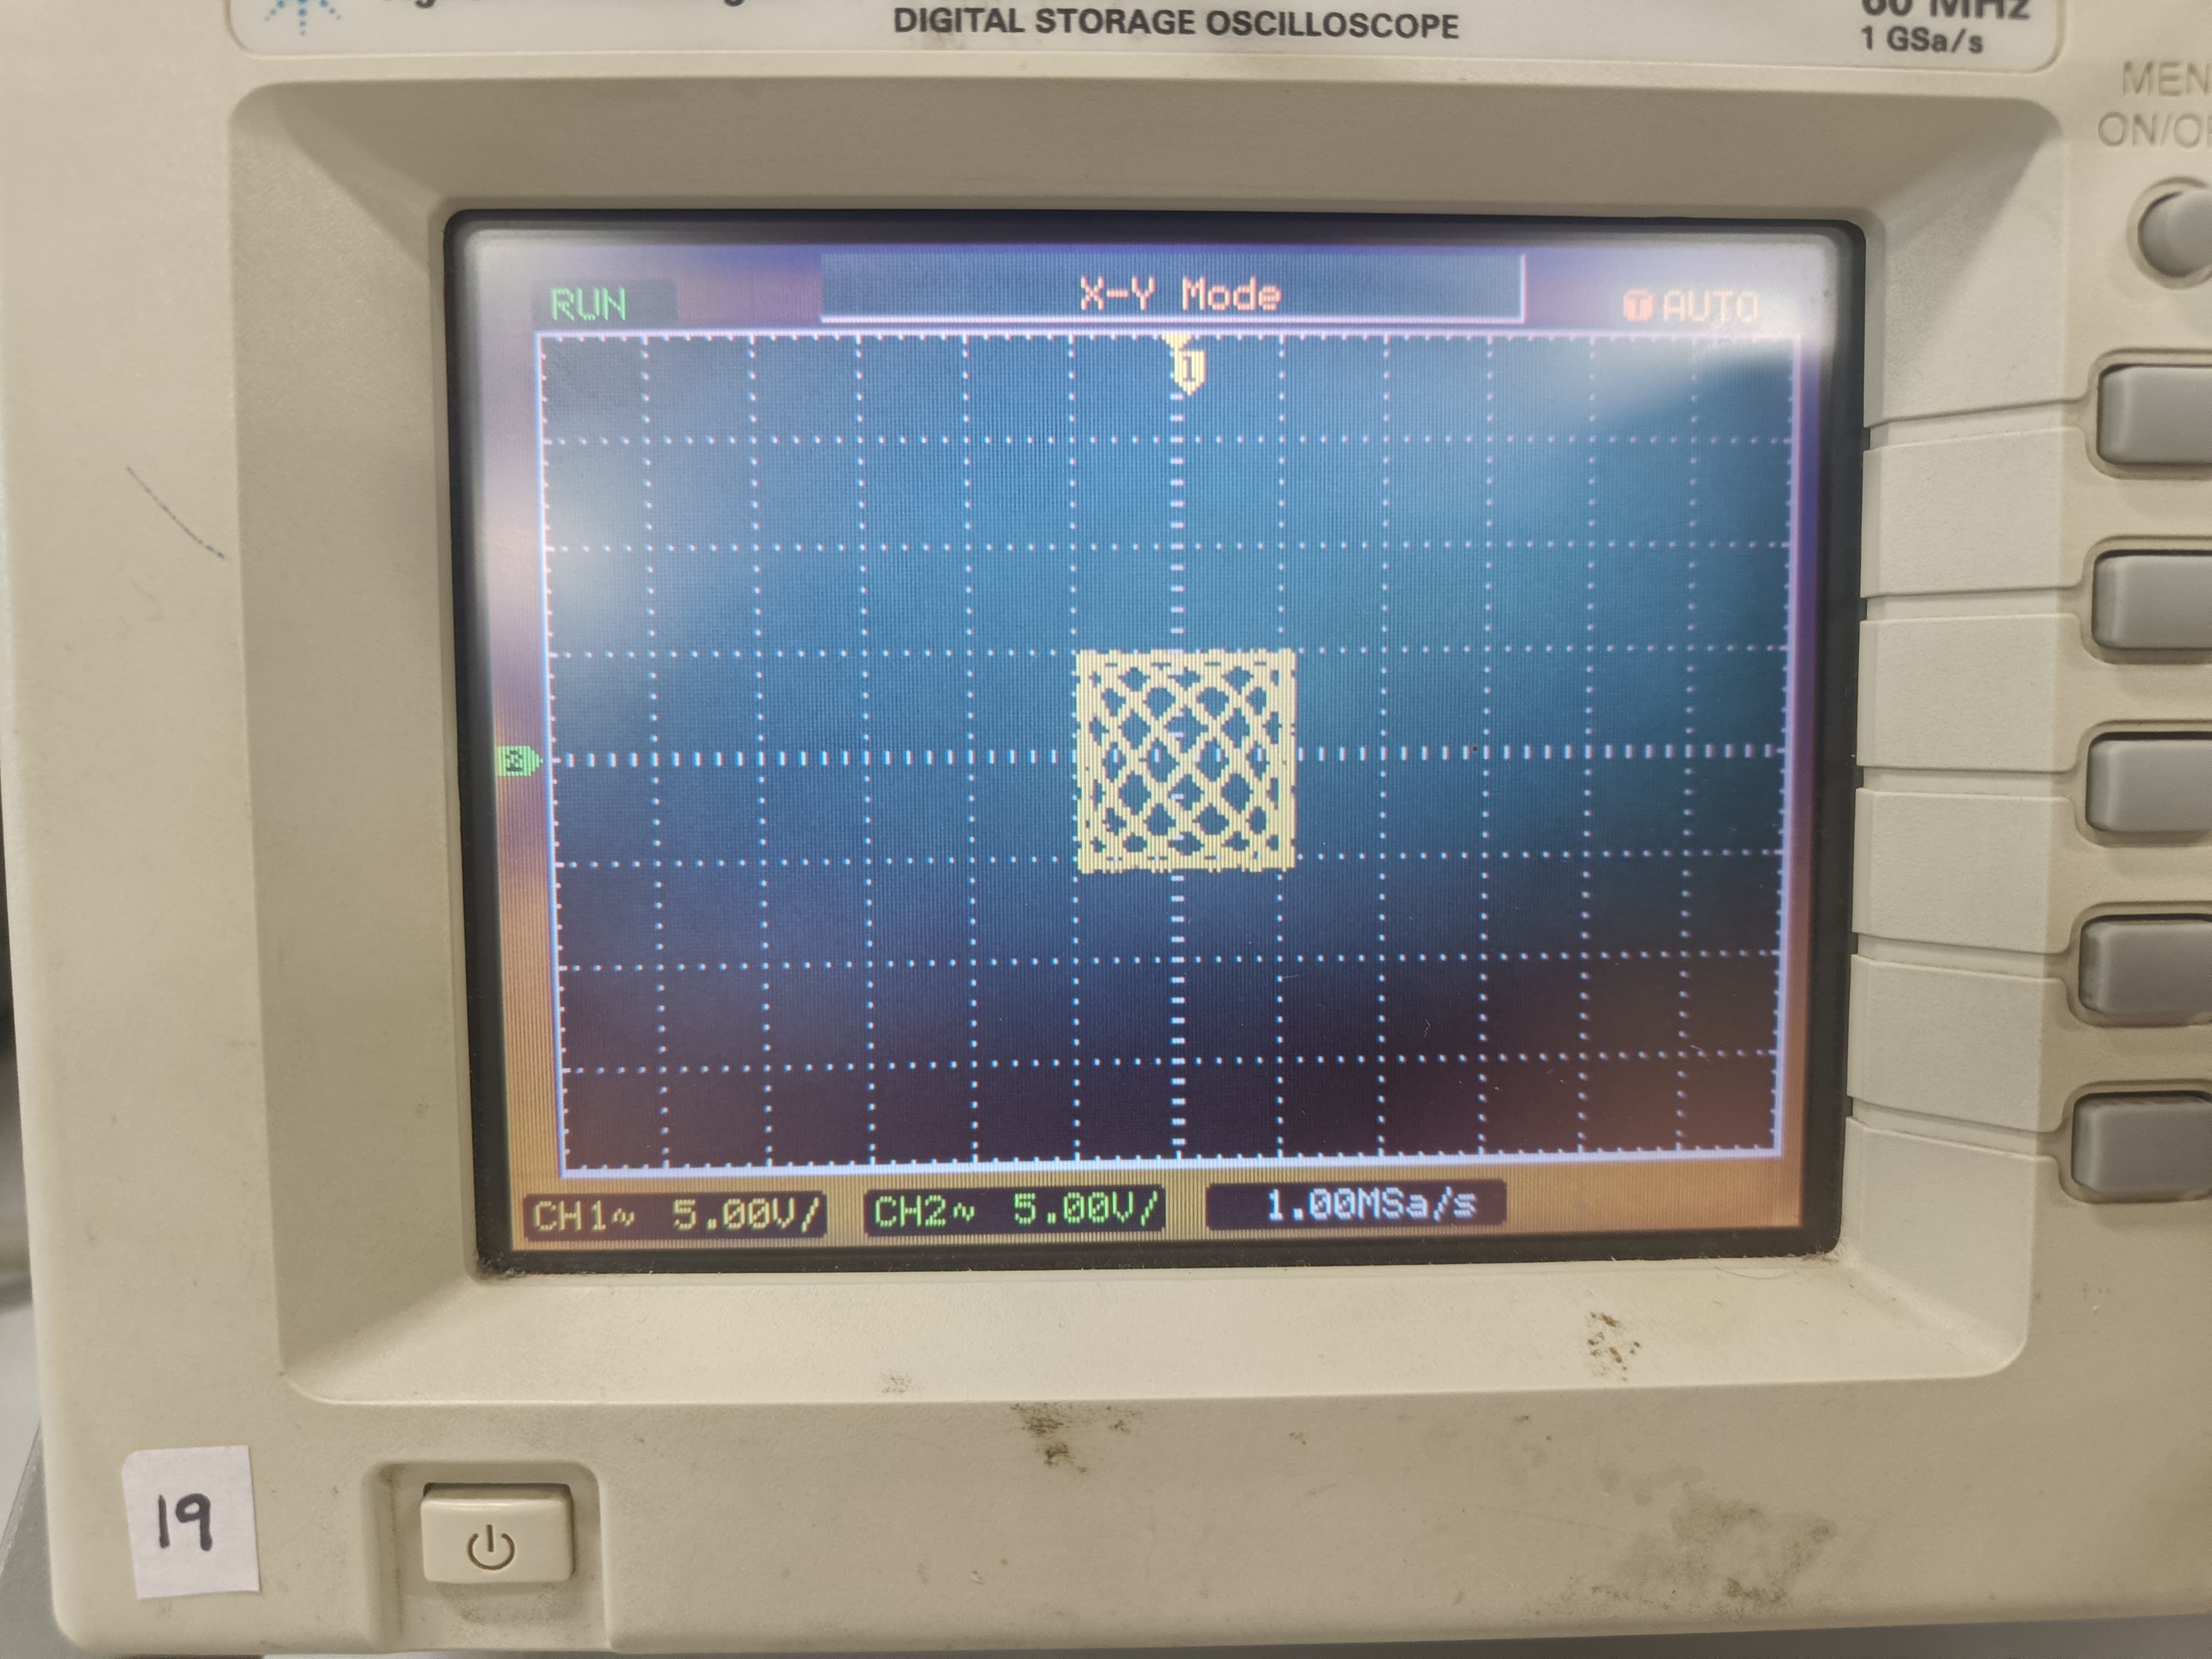
\includegraphics[width=0.7\columnwidth]{pics/WhatsApp Image 2025-01-24 at 11.02.11.jpeg}
        \caption{Output on CRO}
    \end{figure}
    \begin{figure}[H]
        \centering
        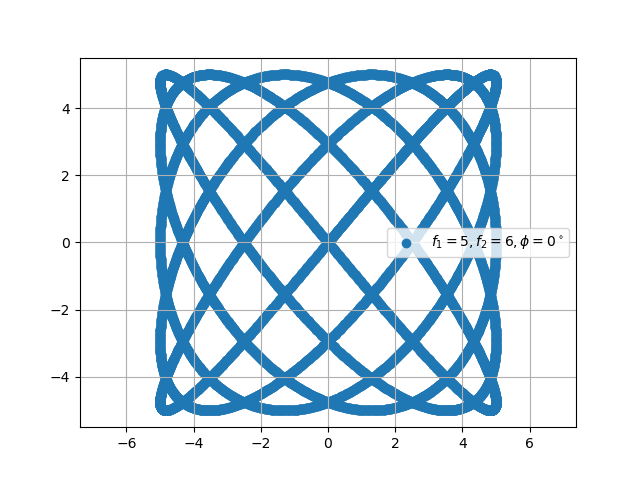
\includegraphics[width=0.7\columnwidth]{figs/fig8.png}
        \caption{Theoretical Plot}
    \end{figure}
\end{enumerate}

\subsection{Capturing an event}
\begin{figure}[H]
    \centering
    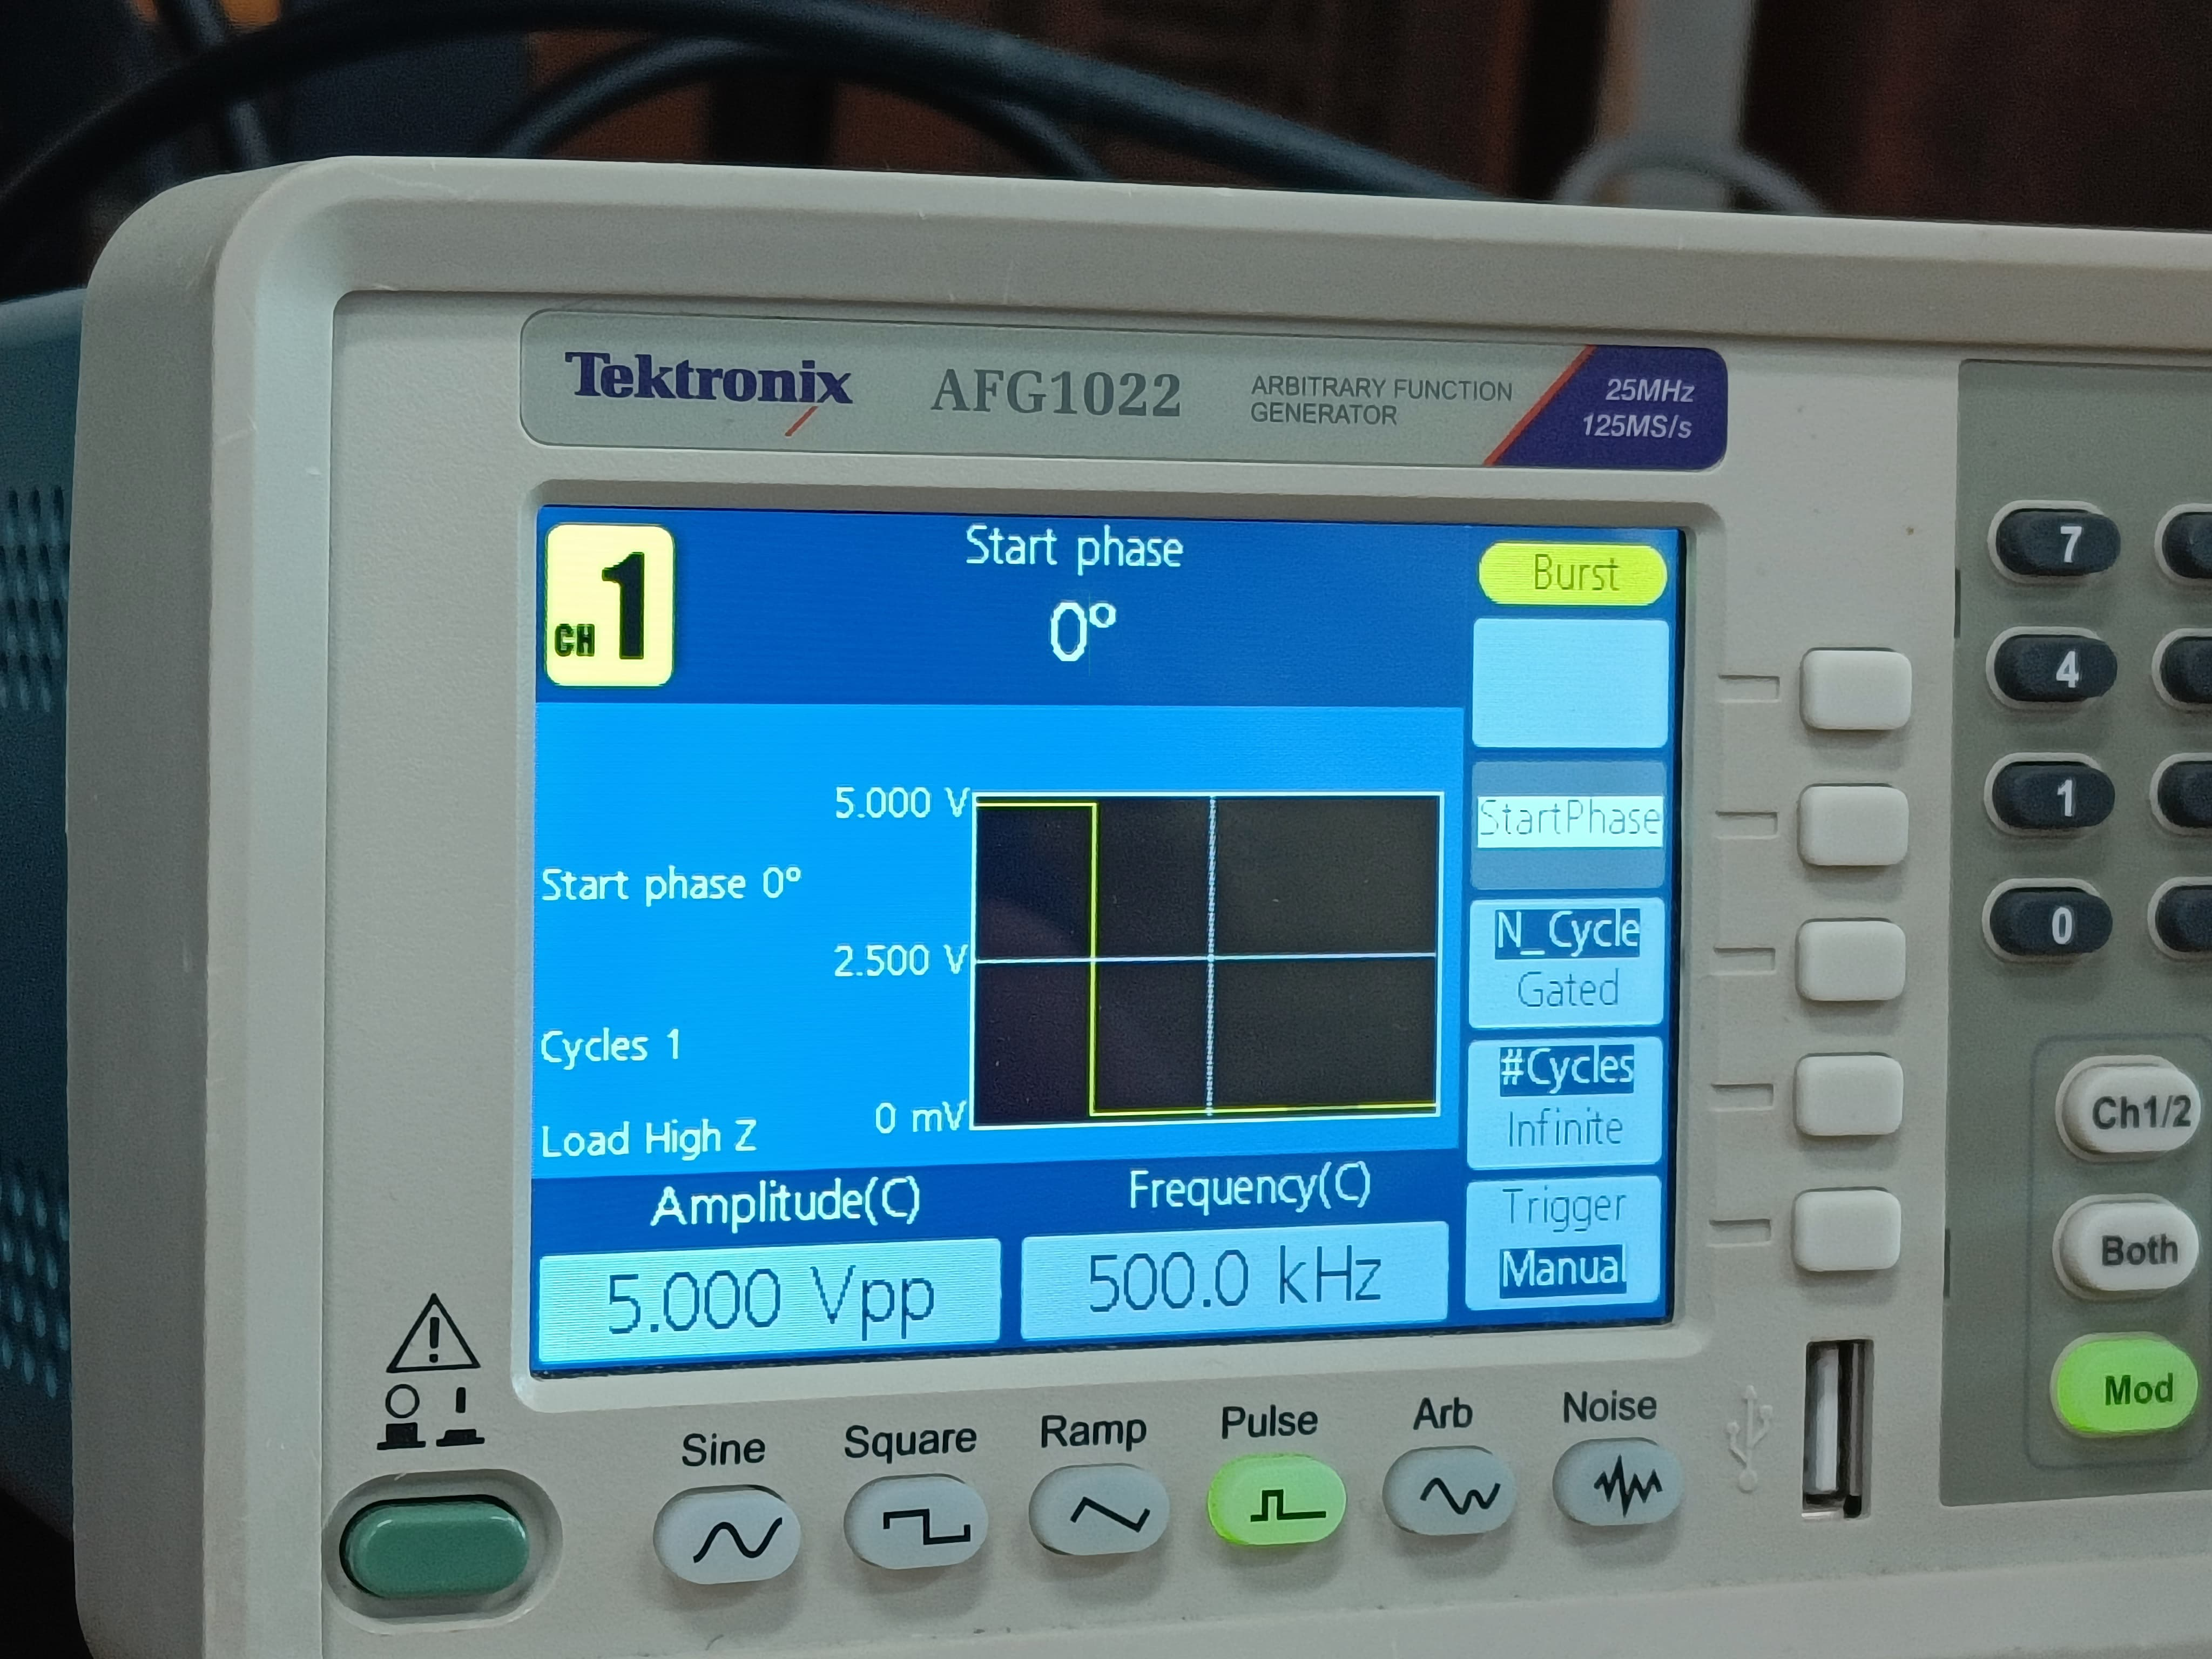
\includegraphics[width=0.7\textwidth]{pics/WhatsApp Image 2025-01-23 at 13.22.08.jpeg}
    \caption{Function Generator}
\end{figure}

\begin{figure}[H]
    \centering
    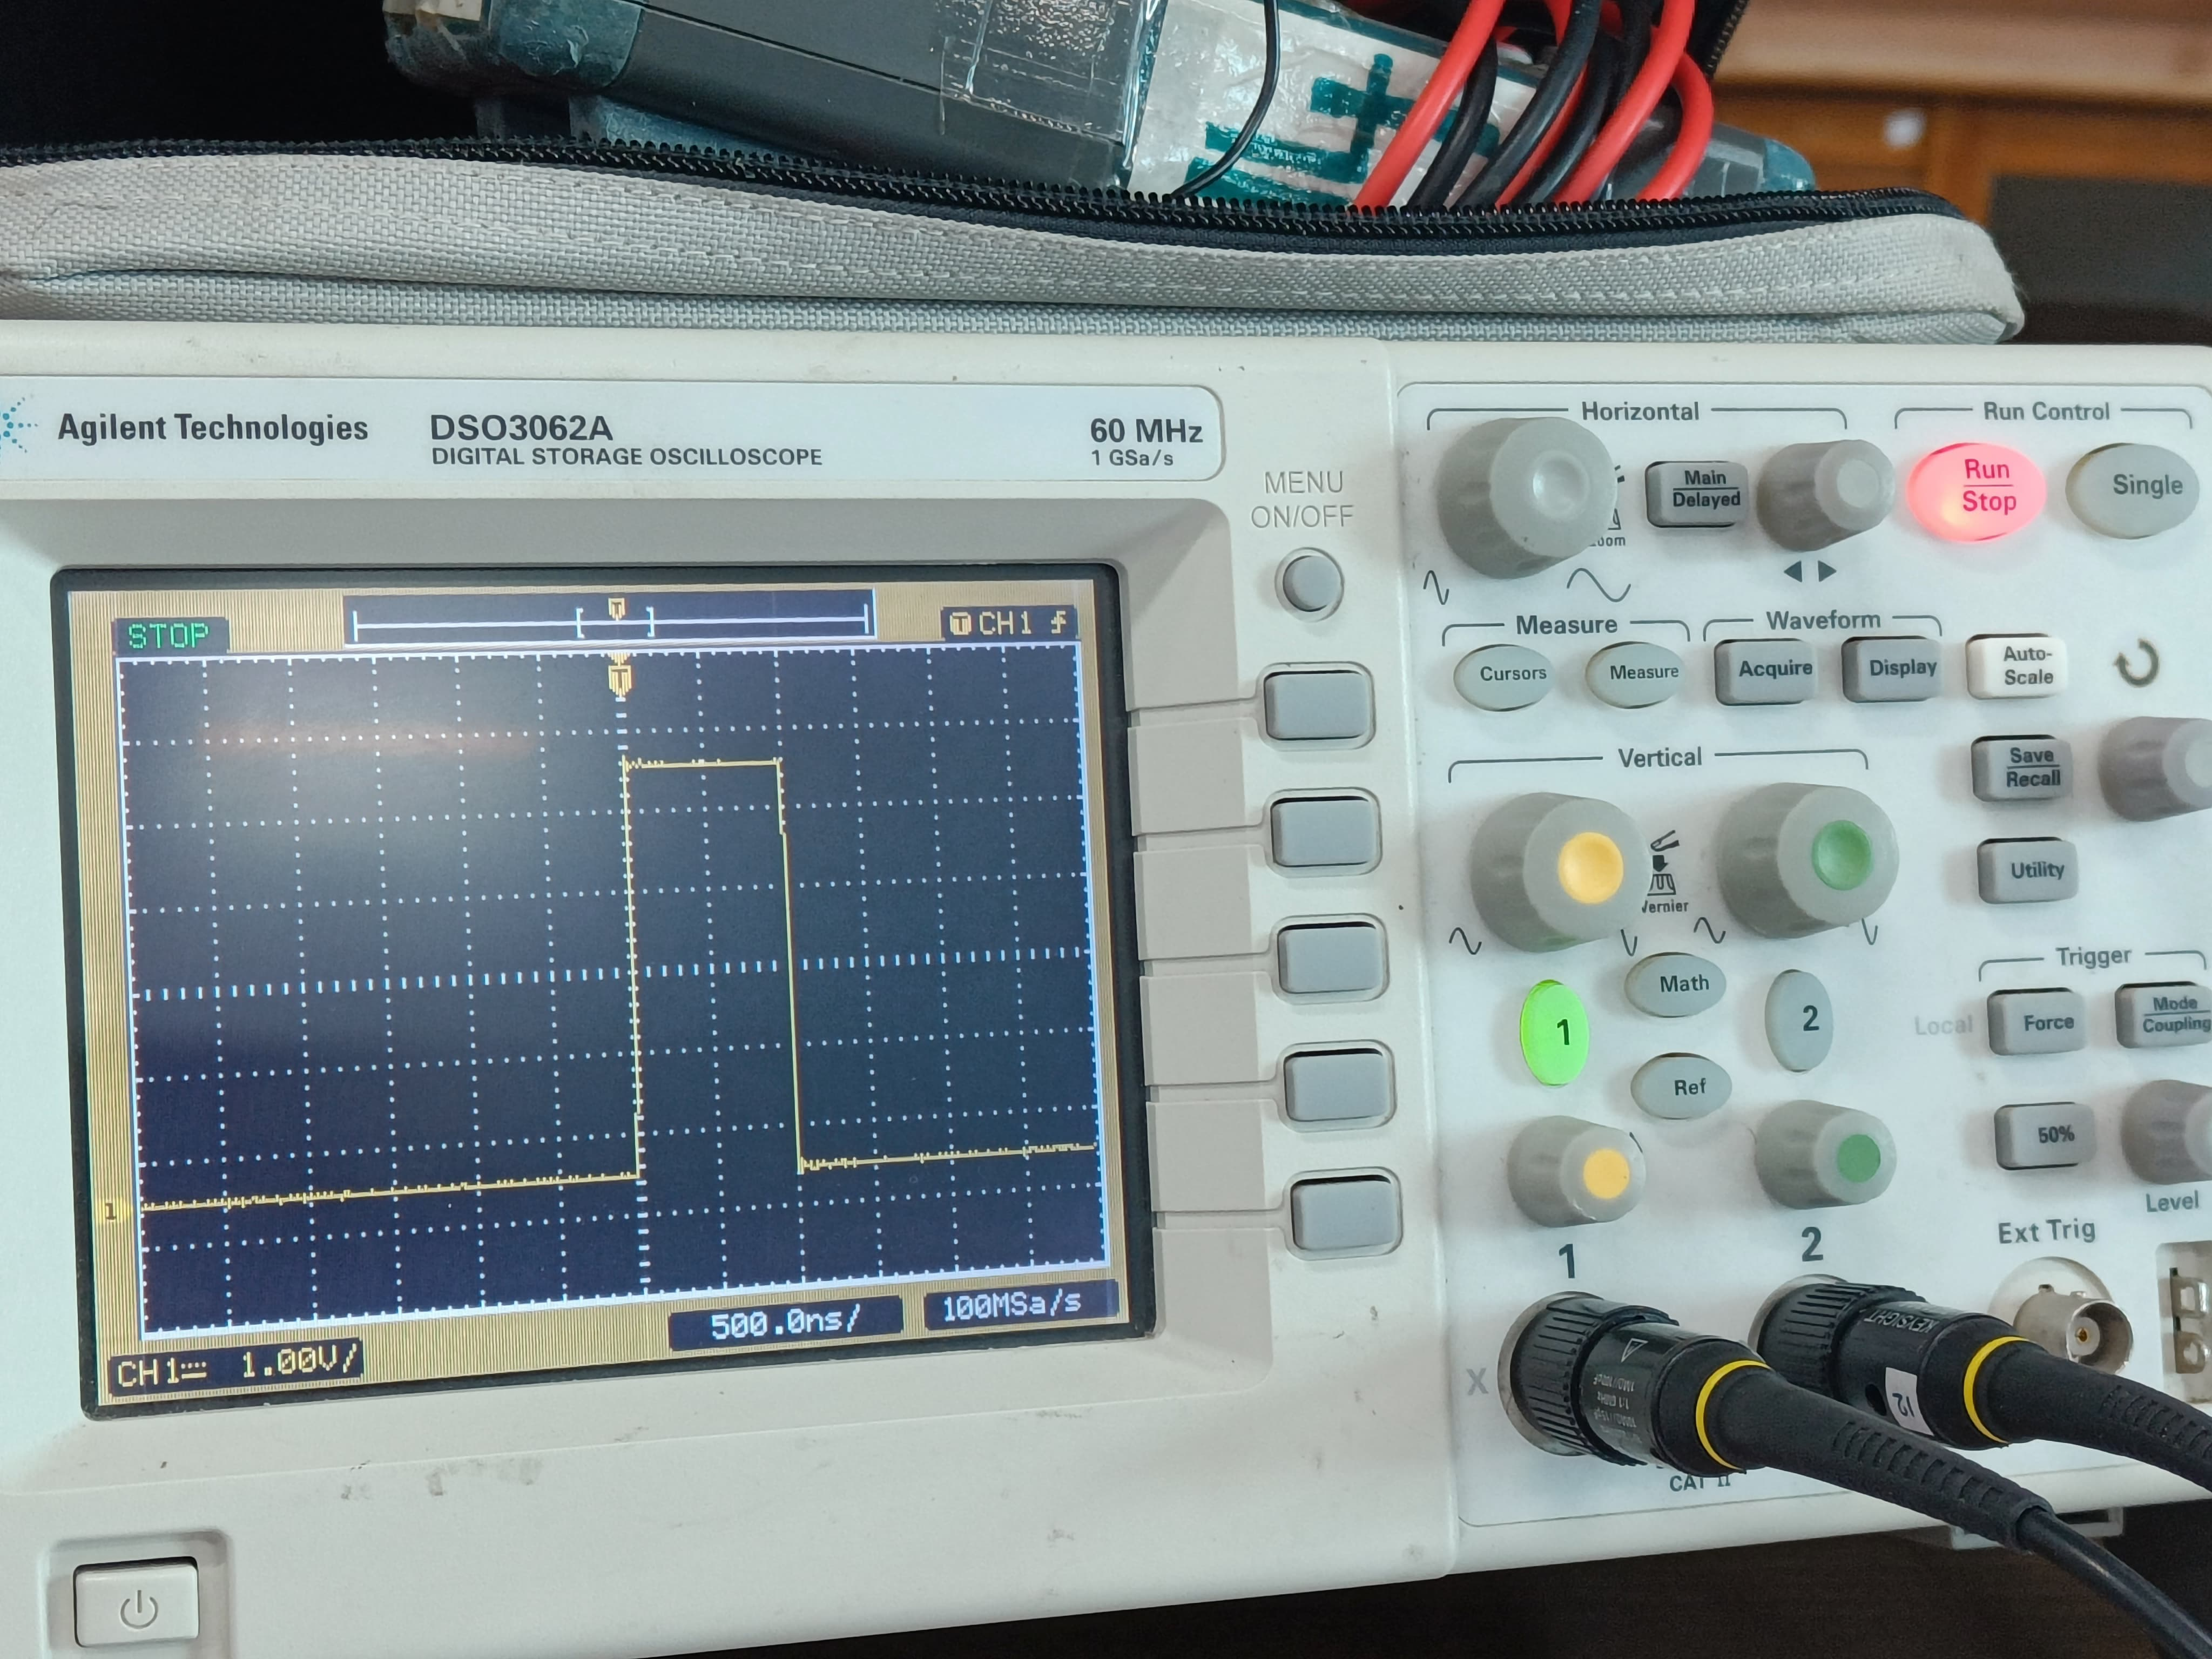
\includegraphics[width=0.7\columnwidth]{pics/WhatsApp Image 2025-01-23 at 13.22.10.jpeg}
    \caption{Signal captured in CRO}
\end{figure}

\section{Precautions}
\begin{enumerate}
    \item Make sure the connections are proper
    \item Join the grounds of the probe and the connector from the CRO and function generator.
    \item Make sure to align phase each time to make changes in the function generator
    \item Make sure the scaling of X and Y are set properly
\end{enumerate}
\end{document}
